\documentclass[11pt]{article}

\usepackage{amsmath,amssymb,amsthm}
\usepackage{mathtools}
\usepackage{bm}
\usepackage{fullpage}
\usepackage{enumitem}
\usepackage{cite}
\usepackage{hyperref}
\usepackage{graphicx}

\newcommand{\R}{\mathbb{R}}
\newcommand{\E}{\mathbb{E}}
\newcommand{\wh}{\widehat}
\newcommand{\wt}{\widetilde}
\newcommand{\Norm}[1]{\left\lVert #1 \right\rVert}
\newcommand{\ip}[2]{\left\langle #1, #2 \right\rangle}
\newcommand{\tr}{\operatorname{tr}}
\newcommand{\diag}{\operatorname{diag}}
\newcommand{\kappaC}{\kappa}
\newcommand{\Pf}{P_f}
\newcommand{\Pa}{P_a}
\newcommand{\Po}{P_o}
\newcommand{\Cf}{\mathcal{B}_f}
\newcommand{\Ca}{\mathcal{B}_a}
\newcommand{\Cg}{\mathcal{B}_g}

\begin{document}

\title{Contract-Driven STAP for Functional Ultrasound: Clinical Profile, Telemetry, and Design Reference}
\author{}
\date{}
\maketitle

\begin{abstract}
We present a fixed, clinical spatiotemporal adaptive processing (STAP) profile for functional ultrasound (fUS) and a contract-driven knowledge-aided (KA) layer that acts only when data support it. The profile freezes tile geometry, temporal aperture, Doppler bands, conditioning targets, and a conditional fast path that applies STAP only on flow-supported tiles. A modality-agnostic contract (R--1/R--2/R--3 plus operator and gating constraints) governs when KA may reshape covariances; sentinels disable KA when alias evidence or headroom is absent. In k-Wave brain fUS simulations (Brain-OpenSkull, Brain-AliasContract, Brain-SkullOR), the frozen STAP PD profile improves low-FPR TPR over MC--SVD/RPCA/HOSVD with 3--5~s/volume latency; KA behaves as a guarded regularizer. On real whole-brain mouse fUS (Mac{\'e}), the hemodynamic variant of the same bands shows contract-consistent telemetry (Pf dominant in $\sim$50\% of atlas H$_1$ tiles vs $\ll$ in H$_0$, lower alias ratios in H$_1$), and an alias-based gate prunes null-tile detections for a PD-z baseline (e.g., 40/7 H$_1$/H$_0$ detections $\rightarrow$ 27/0 at matched TPR). Public Doppler-like datasets (Wang ULM IQ, PICMUS carotid RF) fail the contract (Pf never dominant, flat ROC) and are used only as stress tests, underscoring the need for raw kHz PRF IQ to fully exercise the Doppler KA profile in humans/NHP.
\end{abstract}

\section{Introduction}

We study slow-time detection on fUS tiles with a fixed clinical STAP profile and an explicit contract for when a knowledge-aided (KA) covariance transform may act. Baseline clutter suppression (SVD/MC--SVD/RPCA/HOSVD) yields a whitened slow-time vector $z = \wh R^{-1/2} x$; a temporal STAP core scores tiles in fixed flow/alias bands $(\Pf,\Pa)$ using BR/GLRT-type ratios. KA-STAP applies a band-aware covariance reshape $z' = R_\beta^{-1/2}x = Qz$ but is allowed to act only when regime preconditions and gating/safety sentinels hold.

\paragraph{Contributions.}
\begin{itemize}[nosep]
  \item A frozen clinical STAP PD profile (tile geometry, temporal aperture, Doppler bands, conditioning targets, conditional fast path) that improves low-FPR TPR over MC--SVD/RPCA/HOSVD on k-Wave brain regimes with 3--5~s/volume latency.
  \item A modality-agnostic contract (R--1/R--2/R--3 plus operator, gating, and safety constraints) that makes KA behavior explicit and keeps KA off when evidence or headroom is absent.
  \item Real-data hemodynamic instantiation on Mac{\'e} whole-brain fUS: Pf/alias telemetry matches the contract, and an alias gate prunes null-tile PD-z detections with modest hit loss on visual slices.
  \item Out-of-regime stress tests (Wang ULM IQ, PICMUS carotid RF) where Pf never dominates and ROC is flat; these serve to demonstrate conservative contract behavior and motivate the need for raw kHz PRF IQ in humans/NHP.
\end{itemize}

\subsection*{System overview and contributions}

Algorithmically, the detector we study is not just another clutter filter but a complete slow-time operating regime for functional ultrasound:
\begin{itemize}[nosep]
  \item A fixed, realistic \emph{clinical STAP} profile for brain fUS, in which a motion-compensated SVD clutter filter provides a baseline PD map and an adaptive temporal STAP core operates on small slow-time tiles to improve detection at low false-positive rates. This profile is frozen at design time (tile geometry, temporal aperture, Doppler bands, conditioning targets, training support) and reused unchanged across simulated and real-data regimes.
  \item A \emph{knowledge-aided band transform} that reshapes temporal covariances in flow/alias bands under explicit structural constraints (approximate commutation with band projectors, bandwise scalar gains, bounded anisotropy). This enables alias-aware covariance shaping while retaining predictable behavior on BR/GLRT-type scores.
  \item A \emph{contract-driven, gated KA layer} that only acts in regimes and tiles where the data provide usable alias evidence and baseline headroom: regime-level conditions (R--1/R--2/R--3) define when KA is allowed to act, tile-level gates localize KA to alias-dominated negatives, and safety sentinels (regime sentinel, invariance sentinel, score monotonicity guard) disable KA when assumptions fail or when it would distort high-confidence flow detections.
  \item A \emph{conditional runtime architecture} that separates baseline clutter suppression, temporal STAP, and knowledge-aided transforms. In the clinical configuration, STAP uses a PD-focused GPU fast path and is applied only on tiles that intersect a flow mask; tiles with no flow support retain the baseline PD. This conditional STAP reduces latency by more than an order of magnitude on our k-Wave regimes while preserving PD ROC in the low-FPR band.
  \item A hierarchy of \emph{simulated brain fUS regimes} (motion-and-clutter; alias-augmented contract regimes; skull/OR-inspired regimes) that together exercise the contract: STAP vs SVD/RPCA/HOSVD in realistic motion and clutter, KA-positive behavior in carefully constructed alias-separation regimes, and KA-neutral or guarded behavior in skull/OR-like regimes where alias leaks into $H_1$ or baseline headroom vanishes.
\end{itemize}

The remainder of the document first develops the regime contract and operator-level conditions in a modality-agnostic way, then instantiates them for brain fUS with concrete simulation setups, baselines, and a fixed clinical STAP profile, and finally reports how STAP and KA behave across contract-satisfying and out-of-contract regimes.

Throughout, $H_1$ denotes ``flow'' tiles and $H_0$ background/no--flow tiles.

\subsection*{Notation}

\begin{itemize}[nosep]
  \item Slow--time length $T$. 
  \item Fixed band projectors $\Pf,\Pa,\Po$ in the spectral basis; ranks $d_f, d_a, d_o$.
  \item Baseline covariance estimate $\wh R$; KA blended covariance $R_\beta$.
  \item Baseline whitened tile $z = \wh R^{-1/2}x$. KA whitened tile $z' = R_\beta^{-1/2} x = Qz$.
  \item For a symmetric $A$, band--restricted extreme eigenvalues:
  \[
    \lambda_{\min}(A|_S) := \min_{\substack{v\in\mathrm{ran}(S)\\ \Norm{v}=1}} v^\top A v,\quad
    \lambda_{\max}(A|_S) := \max_{\substack{v\in\mathrm{ran}(S)\\ \Norm{v}=1}} v^\top A v.
  \]
  \item Commutator: $[Q,\Pf] = Q\Pf - \Pf Q$, and similarly for $\Pa$.
\end{itemize}

\section{Results overview}
\label{sec:results-overview}

\begin{itemize}[nosep]
  \item \textbf{Brain-k-Wave simulations (fixed clinical STAP profile).} Across Brain-OpenSkull / Brain-AliasContract / Brain-SkullOR regimes, the frozen clinical STAP PD profile improves low-FPR TPR over MC--SVD/RPCA/HOSVD; conditional STAP yields 3--5~s/volume latency while preserving ROC. KA behaves as a guarded regularizer with no claimed ROC uplift in these regimes.
  \item \textbf{Mac{\'e} whole-brain fUS (hemodynamic variant).} A systematic tile-level sweep over all scans/planes with a fixed hemodynamic STAP configuration finds a small set of mid-visual slices where Pf is dominant in $\approx 0.5$ of H$_1$ tiles versus $\ll 0.25$ in H$_0$ and median $\log(E_{\mathrm{Pa}}/E_{\mathrm{Pf}})$ in H$_1$ is lower by $\approx 0.5$--2; on these contract-positive planes an alias-based gate at TPR $\approx 0.5$ removes roughly one-third of null-tile PD-z detections at $\approx 10$--15\% hit cost (e.g., 40/7 $\rightarrow$ 34/0 and 37/0 $\rightarrow$ 32/0 H$_1$/H$_0$ hits), while being essentially ROC-neutral on other slices.
  \item \textbf{Out-of-regime real datasets.} Wang ULM IQ and PICMUS carotid RF fail the Doppler contract under the frozen bands (Pf peak $\approx 0$, alias flat, ROC flat). They are treated as stress tests only; details in Appendix~\ref{app:negative-real}.
\end{itemize}

\section{Results}
\label{sec:results}

\subsection{Brain-k-Wave regimes: ROC and latency}
The frozen clinical STAP PD profile improves low-FPR detection over MC--SVD/RPCA/HOSVD across Brain-OpenSkull, Brain-AliasContract, and Brain-SkullOR. In the target band (FPR $\approx 10^{-4}$--$10^{-3}$), STAP lifts TPR relative to all baselines; KA is neutral/guarded in these regimes. Conditional STAP (tiles intersecting flow masks only) reduces runtime from tens of seconds to $\approx 3$--$5$~s per volume while preserving PD ROC, enabling near-real-time operation.

\begin{table}[h]
\centering
\begin{tabular}{lcccc}
\hline
Regime & MC--SVD (s) & STAP full (s) & STAP conditional (s) & TPR base / STAP @ $10^{-4}$ \\
\hline
Brain-OpenSkull & $\approx 1.2$ & $\approx 61$ & $\approx 4.7$ & $0.00 / 0.21$ \\
Brain-AliasContract & $\approx 1.0$ & $\approx 45$ & $\approx 3.9$ & $0.00 / 0.17$ \\
Brain-SkullOR & $\approx 1.2$ & $\approx 56$ & $\approx 3.2$ & $0.00 / 0.17$ \\
\hline
\end{tabular}
\caption{Representative latency and low-FPR TPR for the clinical STAP PD profile versus MC--SVD on the main Brain-* regimes. Conditional STAP skips tiles with no flow-mask overlap.}
\label{tab:brain_latency_results}
\end{table}

\subsection{Mac{\'e} whole-brain fUS: hemodynamic contract and gating}
We treat the Mac{\'e}/Urban whole-brain dataset as a PD-only, open-skull analogue of Brain-OpenSkull and run a tile-level hemodynamic STAP analysis with fixed bands $\Pf=[0,0.5]$~Hz, guard $[0.5,1.0]$~Hz, and $\Pa=[1.0,3.0]$~Hz on $8\times 8$ tiles (stride 3) labeled via the Allen atlas (VIS/SC/LGd as H$_1$, CP/CA/DG as H$_0$). A sweep over all six scans and 84 planes shows that hemodynamic Pf/Pa structure is weak on most slices (Pf peak fractions in H$_1$/H$_0$ broadly similar, alias ratios nearly class-invariant), but identifies eight mid-visual planes (including scan1/2 planes 3--4) where Pf is dominant in $\approx 0.45$--0.53 of H$_1$ tiles versus $\approx 0.04$--0.24 in H$_0$ and median $\log(E_{\mathrm{Pa}}/E_{\mathrm{Pf}})$ in H$_1$ is lower than in H$_0$ by $\approx 0.5$--2. On this contract-positive subset, PD-z remains the primary scalar detector and hemo-STAP band-ratio/GLRT behave as neutral cross-checks, but a simple alias-based gate $m_{\mathrm{alias}} = E_{\mathrm{Pa}}/E_{\mathrm{Pf}}$ at TPR $\approx 0.5$ reduces aggregate null-tile detections from 242 to 157 (with H$_1$ hits reduced from 320 to 277). On the canonical visual slice scan1/plane~3, PD-z yields 40 H$_1$/7 H$_0$ detections and alias-gated PD-z yields 34/0; on scan1/plane~4, 37/0 $\rightarrow$ 32/0. Across all 84 planes the same fixed alias gate is essentially ROC-neutral, consistent with treating hemodynamic Pf/Pa as a contract-driven sentinel that only acts where Pf occupancy and alias telemetry indicate an in-regime slice. Figures~\ref{fig:mace_plane3}--\ref{fig:mace_plane4} illustrate Pf peak fraction, alias distributions, and gated detections on two representative mid-visual planes.
\begin{figure}[h]
\centering
\includegraphics[width=0.8\linewidth]{reports/mace_scan1_plane3_gate.png}
\caption{Mac{\'e} scan1 plane3: Pf peak fraction, alias distributions, PD-z map, and detections at TPR$\approx 0.5$ with alias gate overlay (cyan).}
\label{fig:mace_plane3}
\end{figure}
\begin{figure}[h]
\centering
\includegraphics[width=0.8\linewidth]{reports/mace_scan1_plane4_gate.png}
\caption{Mac{\'e} scan1 plane4: Pf peak fraction, alias distributions, PD-z map, and detections at TPR$\approx 0.5$ with alias gate overlay (cyan).}
\label{fig:mace_plane4}
\end{figure}

\subsection{Negative real-data stress tests}
Wang ULM IQ and PICMUS carotid RF: Pf peak $\approx 0$, Po dominates, alias metrics show no class separation, and PD-z/BR/GLRT ROCs are flat under the frozen Doppler bands. Both are classified as out of regime and used only as contract sanity checks (details in Appendix~\ref{app:negative-real}).

\section{Related work}
\label{sec:related}

\textbf{STAP and knowledge-aided STAP.} Classical MVDR/LCMV/STAP and knowledge-aided variants shape covariances using external structure \cite{Capon1969Beamformer,FrostBeamformer, WardSTAPTutorial, GuerciSTAPBook2003,WicksKASTAP2006,MelvinGuerciKAParadigm2006}. Our contract formalizes when such transforms are allowed to act in fUS and keeps them off when data are out of regime.

\textbf{Ultrasound clutter suppression.} SVD clutter filters \cite{Mace2013,Rabut2020,ICDFUS2021}, robust PCA, and higher-order SVD have been used for fUS denoising. We benchmark STAP against MC--SVD, RPCA, and HOSVD baselines in brain-like regimes.

\textbf{fUS detection and hemodynamic analysis.} GLM-based detection and atlas-driven ROI analysis are common in hemodynamic fUS \cite{Demeneglmband2016,UrbanWholeBrain2015}; our hemodynamic STAP variant reuses the same banded temporal machinery on PD time series and adds alias-aware gating as a safety layer.

\section{Discussion and future work}
\label{sec:discussion}

\textbf{What the current results show.} The measured ROC gains come from the fixed clinical STAP PD profile; in all tested regimes KA behaves as a guarded regularizer/sentinel. The hemodynamic Mac{\'e} analysis demonstrates that the same banded machinery and alias telemetry transfer to real PD data and can safely prune null detections; Doppler KA uplift is not observed in available datasets.

\textbf{Data and regime limitations.} Public Doppler-like datasets are post-filtered or low-PRF, so R--1/R--2 fail and KA is rightly disabled. Full evaluation of Doppler KA in humans/NHP requires raw kHz PRF IQ pre-clutter, with known PRF/geometry, to mirror the Brain-* regimes.

\textbf{Future work.} (i) Acquire/run on in-regime clinical/NHP datasets with raw IQ to test Doppler KA under the fixed contract. (ii) Tighten the clinical STAP latency story with hardware-specific implementations. (iii) Explore learned score calibration/gating trained in simulation and frozen for deployment as a light-weight KA alternative.

\section{KA Contract (Modality--Agnostic)}

In this part we describe a regime contract and operator-level conditions for a knowledge-aided temporal covariance transform layered on top of a baseline slow-time detector. The contract is formulated in terms of abstract band projectors $(\Pf,\Pa,\Po)$, alias scores, and score distributions, and does not depend on any particular imaging modality. Only in later sections do we instantiate these conditions for functional ultrasound (fUS) brain imaging with concrete band choices, acquisition parameters, and baselines.

\subsection{Regime Preconditions (Data--Level, Non--Negotiable)}
\label{sec:regime}

The most important empirical lesson is: even if the KA operator $Q$ and band design $(\Pf,\Pa)$ are perfect in an abstract sense, \emph{uplift requires the data themselves to be in a compatible regime}. This section codifies that.

We write $S(f)$ for the (multi--taper) PSD of a baseline--whitened tile, and define
\[
E_f := \sum_{f\in\Cf} S(f),\quad
E_a := \sum_{f\in\Ca} S(f),\quad
E_g := \sum_{f\in\Cg} S(f),
\]
with $\Cf,\Ca,\Cg$ the flow, alias, and guard bands in frequency.

\subsection{R--1: Band Occupancy Separation}

We require that the fixed bands $(\Cf,\Ca)$ are physically meaningful for the current PRF, slow--time length $T$, and DPSS parameters, in the sense that label statistics show actual occupancy.

On a held--out labeled sample:
\begin{align}
\mathbb{P}\!\left\{f_{\mathrm{peak}}\in\Cf \;\middle|\; H_1\right\} &\ge p_{f,\min},\qquad p_{f,\min}\in [0.5,0.7],\\[0.5ex]
\mathbb{P}\!\left\{f_{\mathrm{peak}}\in\Ca \;\middle|\; H_0\right\} &\ge p_{a,\min},\qquad p_{a,\min}\in [0.2,0.3],
\end{align}
where $f_{\mathrm{peak}}$ is the frequency at which $S(f)$ attains its maximum and $H_1$/$H_0$ denote flow/background tiles.

Interpretation: a majority of flow tiles have their dominant PSD peak \emph{inside} the flow band, and a nontrivial fraction of background tiles have their dominant peak in the alias band. This ensures that the band projectors $(\Pf,\Pa)$ actually correspond to distinct physical processes.

\paragraph{Implementation in Brain--* clinical profiles.}
For the Brain--OpenSkull / Brain--AliasContract / Brain--SkullOR clinical regimes, the raw k-Wave RF tensor $x(t,\text{angle},\text{element})$ lives on an angle/element grid that does not align pixelwise with the STAP PD masks $(\text{Ny}\times\text{Nx})$. In these cases we implement R--1 via the whitened multi--taper PSD / band--ratio telemetry computed on the \emph{same} spatial grid as the PD maps: $f_{\mathrm{peak}}$ is taken from the whitened PSD peaks used in the band--ratio recorder, and we report $P(f_{\mathrm{peak}}\in\Cf\mid H_1)$ and $P(f_{\mathrm{peak}}\in\Ca\mid H_0)$ from those tilewise peak statistics. When the RF tensor is spatially aligned with the masks (e.g.\ 1D pilots), we instead use a direct FFT on $x(t,\cdot,\cdot)$ as in the definition above.

\subsection{R--2: Alias Score Class Separation}

We generalize the alias metric used for gating.

\paragraph{Alias score.} Let $m_{\text{alias}}(z)$ be any scalar score derived from the baseline PSD and/or covariance satisfying:
\begin{itemize}[nosep]
  \item $m_{\text{alias}}$ increases when $E_a$ grows relative to $E_f$,
  \item $m_{\text{alias}}$ is larger when Pa energy is more coherent or concentrated (e.g.\ a strong tone),
  \item $m_{\text{alias}}$ is penalized when guard/edge energy $E_g$ is large.
\end{itemize}
Examples (not exhaustive):
\begin{itemize}[nosep]
  \item Log band ratio: $m_{\text{alias}}(z) = \log\frac{E_a+\epsilon}{E_f+\epsilon}$,
  \item Combination of band fractions: $m_{\text{alias}}(z) = \frac{E_a}{E_f+E_a+E_g} \cdot c_a$ where $c_a$ is an alias--band coherence metric (e.g.\ leading eigenvalue fraction of a band--restricted covariance),
  \item Peak--location based scores (peak in Pa, high tone prominence).
\end{itemize}

For KA to be meaningfully guided by alias evidence, we require \emph{class--differential separation} of $m_{\text{alias}}$:
\begin{equation}
\label{eq:R2}
\operatorname{median}\!\left(m_{\text{alias}}\mid H_0\right) - \operatorname{median}\!\left(m_{\text{alias}}\mid H_1\right) \;\ge\; \Delta_{\min},
\end{equation}
with $\Delta_{\min}$ set so that alias dominance differs by at least a factor $\approx e^{\Delta_{\min}}$ in expectation (for log ratio, $\Delta_{\min}\approx 0.3$ corresponds to a $\approx 35\%$ relative difference in $E_a/E_f$ medians).

If \eqref{eq:R2} fails (alias score almost identical on $H_0$ and $H_1$), the alias gate (Section~\ref{sec:gating}) has no reliable signal and KA uplift cannot be expected.

\subsection{R--3: Baseline Headroom}

Let $S^-$ be the baseline score distribution on negatives, and $\text{pAUC}_\text{base}(\alpha)$ be the partial AUC up to FPR $\alpha$.

We require:
\begin{itemize}[nosep]
  \item Sufficient \emph{quantile density} at the target FPR $\alpha$ (as already assumed implicitly in SL--2): the density $f_-(t_\alpha)$ at the $\alpha$--quantile $t_\alpha$ is bounded away from 0.
  \item Baseline not already numerically saturated: for a chosen $\alpha_{\max}$ (e.g.\ $10^{-3}$),
  \[
    \text{pAUC}_\text{base}(\alpha\le \alpha_{\max}) \le \text{pAUC}_{\max} - \varepsilon_{\text{AUC}},\qquad \varepsilon_{\text{AUC}}>0,
  \]
  where $\text{pAUC}_{\max}$ is the ideal partial AUC under perfect separation.
\end{itemize}

If the baseline already achieves near--maximal pAUC at the FPR of interest, even a perfect KA transform cannot provide significant gains; in this regime KA can serve as a regularizer or safety mechanism, but not as a source of measurable uplift.

\subsection{Operator--Level Sufficient Structure (Non--Negotiable Core)}
\label{sec:operator}

This section is unchanged at the core: it describes conditions on $Q$ alone under which KA behaves like a band--wise scalar rescaling of scores, up to small perturbations.

\subsection{OC--1: Approximate Band Commutation}

We require $Q$ to be nearly block--diagonal with respect to $(\Pf,\Pa,\Po)$:
\[
\Norm{[Q,\Pf]}_2 \le \varepsilon_{\text{mix}},\qquad
\Norm{[Q,\Pa]}_2 \le \varepsilon_{\text{mix}},
\]
for some small $\varepsilon_{\text{mix}}\in[0,1)$ (typical target $\le 0.05$).

Interpretation: $Q$ preserves band subspaces up to small mixing; it does not rotate energy from Pf into Pa or vice versa in any substantial way. This rules out the failure mode where KA accidentally feeds alias into the flow numerator.

\paragraph{Runtime label--free check.}
Let $\wh Q := R_\beta^{-1/2}\wh R^{1/2}$ be the realized KA transform. Estimate
\[
\wh\varepsilon_{\text{mix}} :=
\max\left\{ 
  \frac{\Norm{\Pf \wh Q \Pa}_F}{\Norm{\Pf \wh Q \Pf}_F},
  \frac{\Norm{\Pa \wh Q \Pf}_F}{\Norm{\Pa \wh Q \Pa}_F}
\right\},
\]
and require $\wh\varepsilon_{\text{mix}} \le \varepsilon_{\text{mix}}$.

\subsection{OC--2: Differential Band Gains with Spectral Bounds}

We require that $Q^\top Q$ is well approximated by bandwise scalars on the ranges of $\Pf,\Pa,\Po$, i.e., there exist $s_f,s_a,s_o>0$ and tolerances $\delta_f,\delta_a,\delta_o\in[0,1)$ such that
\begin{align*}
  &s_f^2(1-\delta_f)\,\Pf \preceq \Pf Q^\top Q \Pf \preceq s_f^2(1+\delta_f)\,\Pf,\\
  &s_a^2(1-\delta_a)\,\Pa \preceq \Pa Q^\top Q \Pa \preceq s_a^2(1+\delta_a)\,\Pa,\\
  &s_o^2(1-\delta_o)\,\Po \preceq \Po Q^\top Q \Po \preceq s_o^2(1+\delta_o)\,\Po,
\end{align*}
with \emph{strict separation}
\[
\frac{s_a}{s_f} \ge \Lambda > 1 + c\,\varepsilon_{\text{mix}},\qquad c\in[2,4].
\]

Interpretation: within each band, $Q^\top Q$ behaves like a scalar ($s_f^2,s_a^2,s_o^2$) up to modest anisotropy $\delta_\bullet$, and the alias band gains are strictly larger than flow band gains.

\paragraph{Runtime label--free check.}
Compute eigenvalues of the band--projected operators:
\[
\lambda_{\min}^f,\lambda_{\max}^f := \lambda_{\min/\max}(Q^\top Q|_{\Pf}),
\]
and similarly for $a,o$. Set
\[
\wh s_f^2 := \tfrac12(\lambda_{\min}^f + \lambda_{\max}^f),\quad
\wh\delta_f := \frac{\lambda_{\max}^f - \lambda_{\min}^f}{\lambda_{\max}^f + \lambda_{\min}^f},
\]
and analogously for $\wh s_a,\wh s_o$ and $\wh\delta_a,\wh\delta_o$. Require $\wh\delta_\bullet\le\delta_\bullet$ and $\wh s_a/\wh s_f \ge \Lambda$.

\subsection{Consequence: Approximate Multiplicative Effect on Scores}

Under OC--1--OC--2, for any $z$ one has
\[
\mathrm{BR}(Qz) = \frac{z^\top Q^\top \Pf Q z}{z^\top Q^\top \Pa Q z}
  \approx \frac{s_f^2}{s_a^2} \cdot \mathrm{BR}(z) \cdot (1+\Delta_{\text{BR}}(z))
\]
with $|\Delta_{\text{BR}}(z)| \le C_1(\delta_f+\delta_a) + C_2 \varepsilon_{\text{mix}}$, for constants $C_1,C_2$ depending only on band dimensions. A similar approximation holds for $\mathrm{GLRT}_\rho(z)$ with denominators involving $s_a^2,s_o^2$.

Thus, if $\Lambda = s_a/s_f>1$ and tolerances are small, BR/GLRT on a tile are rescaled approximately by a \emph{bandwise constant} factor, with predictable sign (e.g.\ downwards when $s_a>s_f$).

\subsection{Band Geometry \& Leakage Budget}
\label{sec:band-geometry}

This section remains as in the original doc: its role is to ensure that the projectors $\Pf,\Pa$ correspond to well--separated spectral bands given the PRF, $T$, and DPSS parameters, using DPSS tapers and multi-taper spectral estimates in the sense of Slepian and Thomson \cite{SlepianDPSS1978,ThomsonMTM1982,PercivalWaldenSAPABook1993}.

\subsection{BG--1: Leakage Separation Margin}

Let $G(f,g)$ be the multi--taper spectral leakage kernel associated with your DPSS design (known from design). Require
\[
\max_{f\in\Cf} \sum_{g\in\Ca} G(f,g) \le \ell_{\max},\qquad \ell_{\max} \le 0.15.
\]

Interpretation: at most 15\% of energy from an on--grid flow bin leaks into the alias band, and vice versa. This supports keeping the band mixing in OC--1 small after whitening.

\subsection{BG--2: Band--Edge Guard}

Define a guard band $\Cg$ separating $\Cf$ and $\Ca$ such that
\[
\mathrm{dist}(\Cf,\Ca) \ge b_g,
\]
for some guard width $b_g$ in frequency (or bins). Require that any energy within $b_g$ of $\Cf$ leaks only modestly into $\Ca$:
\[
\sum_{g:\,\mathrm{dist}(g,\Cf)\le b_g} G(f,g) \le \ell_{\text{edge}},\qquad \ell_{\text{edge}}\le 0.1.
\]

Interpretation: avoid designing $\Cf,\Ca$ so tightly that off--grid peaks straddle the boundary; the guard ensures band--edge leakage is limited.

\subsection{BG--3: Within--Band Condition Numbers}

From the baseline whitened covariance in each band, require
\[
\kappa_f := \frac{\lambda_{\max}(\wh R|_{\Pf})}{\lambda_{\min}(\wh R|_{\Pf})} \le \kappa_f^{\max},\qquad
\kappa_a := \frac{\lambda_{\max}(\wh R|_{\Pa})}{\lambda_{\min}(\wh R|_{\Pa})} \le \kappa_a^{\max},
\]
with $\kappa^{\max}\in[10,40]$ depending on $T$ and sample support.

Interpretation: this makes it feasible to construct $R_\beta$ that achieves OC--2 with moderate $\beta,\delta$ without overly crushing the flow band.

\subsection{Covariance blending and gating (summary)}
\label{sec:cov-blending}

KA reshapes covariances only within bands. We use either a commuting band-scalar transform with target gains $(s_f,s_a,s_o)$ or a trace-normalized blend $R_\beta$ with small diagonal lift; both enforce bandwise structure (no off-block priors). Gating localizes KA to alias-dominated, low-coverage tiles using alias scores, guard ratios, optional flow coherence/coverage checks, baseline score windows, depth/PD/registration cues, and is validated via coverage rates $p_-,p_+$. Full definitions and thresholds are provided in Appendix~\ref{app:alg-details}.

\subsection{Score--Level Guarantees}
\label{sec:score-level}

This section is unchanged in structure; we only make the dependence on $p_-,p_+$ explicit.

\subsection{SL--1: Per--Tile Multiplicative Effect}

Under OC--1--OC--2, for any $z$,
\[
\mathrm{BR}_{\text{KA}}(z) = \mathrm{BR}(Qz) 
  \approx \frac{s_f^2}{s_a^2} \cdot \mathrm{BR}_{\text{base}}(z) \cdot (1 + O(\delta_\bullet+\varepsilon_{\text{mix}})).
\]

Similarly,
\[
\mathrm{GLRT}_{\rho,\text{KA}}(z) \approx 
  \frac{s_f^2}{\alpha_a(z)\,s_a^2 + \alpha_o(z)\,s_o^2}\cdot \mathrm{GLRT}_{\rho,\text{base}}(z),
\]
where
\[
\alpha_a(z) := \frac{z^\top \Pa z}{z^\top(\Pa+\rho I)z} \in [0,1],\quad
\alpha_o(z) := \frac{\rho\Norm{z}^2}{z^\top(\Pa+\rho I)z}\in[0,1].
\]

On alias--dominant tiles (large $\alpha_a(z)$), both BR and GLRT are approximately multiplied by $\mu := s_f^2/s_a^2<1$.

\subsection{SL--2: Tail Threshold Improvement at Fixed FPR}

Let $S^-_{\text{base}}$ be the baseline negative score distribution, with CDF $F_-$. Let $t_\alpha$ be the $\alpha$--quantile: $F_-(t_\alpha) = 1-\alpha$. After KA with gating, the negative CDF becomes a mixture:
\[
F'_-(t) = (1-p_-) F_-(t) + p_- F_-(t/\mu),
\]
ignoring higher--order mixing terms and assuming $\mu<1$ is the multiplicative shrinkage factor on gated negatives. Under mild regularity and for $\alpha$ in the low--FPR regime,
\[
t'_\alpha \approx t_\alpha - \frac{p_-(1-\mu)}{f_-(t_\alpha)},
\]
so that $t'_\alpha < t_\alpha$ whenever $p_->0$ and $\mu<1$.

Interpretation: scaling down a fraction $p_-$ of top--tail negatives is equivalent to removing mass from the negative tail; the induced quantile shift moves $t_\alpha$ left, permitting a lower decision threshold at fixed FPR and thereby increasing TPR, provided $p_+$ (positive gating rate) is small.

We emphasize that the SL--2 guarantee is conditioned on:
\begin{itemize}[nosep]
  \item Regime preconditions R--1/R--2/R--3,
  \item Gating coverage in the range $0.2\le p_-\le 0.5$, $p_+\le 0.1p_-$.
\end{itemize}

\subsection{SL--3: Positive Collateral Bound}

Let $p_+$ be the positive gating rate and assume gated positives suffer at most a multiplicative drop $\nu := s_f^2/s_a^2\cdot(1+O(\delta_\bullet+\varepsilon_{\text{mix}}))$. For any threshold $t'_\alpha$ satisfying $F'_-(t'_\alpha)=1-\alpha$, the TPR under KA satisfies
\[
\mathrm{TPR}_{\text{KA}}(t'_\alpha) \ge \mathrm{TPR}_{\text{base}}(t_\alpha) - \eta\,\Phi(\nu),
\]
where $0\le \eta\lesssim \frac{p_+}{p_-}$ (up to geometry) and $\Phi(\nu)$ is the fraction of positives near $t'_\alpha$ that are moved below the threshold. For $p_+\ll p_-$ and $\nu$ close to $1$, the loss term is dominated by the gain from SL--2.

\subsection{Evaluation Discipline}
\label{sec:eval}

This section remains as in the original document: it covers GLRT parameter sharing, block/cluster--aware tail CIs, and effective negatives. These aspects ensure fair comparison but do not themselves cause uplift.

\subsection{Telemetry and Pass/Fail Checklist}
\label{sec:telemetry}

At runtime, label--free telemetry must support the following checks:

\begin{enumerate}[label=(\roman*),nosep]
  \item Band design: BG--1/BG--2/BG--3 satisfied for current DPSS/PRF/$T$.
  \item KA operator: $\wh\varepsilon_{\text{mix}}\le\varepsilon_{\text{mix}}$ (OC--1); $\wh s_a/\wh s_f\ge\Lambda$ and $\wh\delta_\bullet\le 0.1$ (OC--2).
  \item Gating primitives: alias score $m_{\text{alias}}$, guard ratios, flow coverage, FPC, depth, PD, registration; gate $g$ constructed via G--1/G--2/G--2'/G--3/G--4.
  \item Invariance sentinel: if $\wh s_a/\wh s_f\in[1-\epsilon,1+\epsilon]$ with $\epsilon\le 0.02$, KA is effectively a scalar; disable it (see Section~\ref{sec:regime-sentinel}).
\end{enumerate}

\subsection{Regime Sentinel and Safety Guard}
\label{sec:regime-sentinel}

Experience shows that even when OC/BG/CB/G conditions are roughly satisfied, there can exist regimes where KA is either inert or harmful (e.g.\ alias metric flat, gate never fires or fires everywhere, baseline ROC saturated). This section formalizes when KA should be \emph{explicitly disabled}.

\subsection{RS--1: Regime Sentinel (Design--Time)}

On a held--out labeled configuration, check:

\begin{itemize}[nosep]
  \item \textbf{RS--1a: Band occupancy.} If R--1 fails (e.g.\ most flow peaks near DC instead of Pf, or alias peaks rarely in Pa), the band design is not physically realized; do not deploy KA.
  \item \textbf{RS--1b: Alias separation.} If R--2 fails (alias scores $m_{\text{alias}}$ show negligible difference between classes), alias gating has no reliable signal; do not deploy KA.
  \item \textbf{RS--1c: Gating coverage.} If, after choosing $q_{\text{alias}},c_{f,\max},c_{\text{pc}}$, the empirical gating rates satisfy $p_-\approx 0$ or $p_-\approx 1$, or $p_+ \approx p_-$, then gating is either inert, global, or non--differential; do not expect uplift and disable KA by default.
  \item \textbf{RS--1d: Baseline saturation.} If $\text{pAUC}_\text{base}$ in the target FPR range is already at or near maximum and the score ratio distribution under KA has median close to 1 with tiny spread, you are in a ROC--invariant regime; KA can be left off.
\end{itemize}

\subsection{Safety--1: Score Monotonicity Guard (Runtime)}

Even when regime preconditions and gating coverage hold, we require that KA does not produce grossly pathological score transformations on \emph{gated flow tiles}. Let $S_{\text{base}},S_{\text{KA}}$ denote baseline and KA scores on the chosen metric (BR or GLRT).

For the set of gated flow pixels (gated flow tiles), define
\[
r_i := \frac{S_{\text{KA}}(i)}{\max(S_{\text{base}}(i),\varepsilon)},\quad
u_i := \log r_i,
\]
with a small $\varepsilon>0$.

Let
\[
\mathrm{median}_f := \operatorname{median}(u_i),\quad
\mathrm{IQR}_f := Q_{0.75}(u_i) - Q_{0.25}(u_i),
\]
and $\tau_f$ the Kendall $\tau$ rank correlation between $S_{\text{KA}}$ and $S_{\text{base}}$ on these pixels.

We require:
\begin{itemize}[nosep]
  \item \textbf{Sample size.} Apply the guard only if the number of gated flow pixels exceeds a threshold $N_{\min}$ (e.g.\ $N_{\min}=200$). If not, mark KA as ``too sparse to evaluate'' but do not disable it solely on this basis.
  \item \textbf{Flow monotonicity.} KA is marked unsafe if either
  \begin{align*}
    &\mathrm{IQR}_f > \log 10\quad\text{(heterogeneity }>\times10\text{)},\quad\text{or}\\
    &\mathrm{median}_f > \log 10\quad\text{and}\quad |\tau_f| < 0.1,
  \end{align*}
  i.e.\ if KA systematically boosts flow scores by more than an order of magnitude while destroying rank consistency, or applies extremely heterogeneous multiplicative effects.
\end{itemize}

If Safety--1 fails, KA is disabled at runtime for that configuration and the system falls back to pure STAP.

\subsection{What the Regime Does Not Promise (Updated)}

KA--STAP may \emph{fail to provide uplift} or may be disabled by the regime sentinel / safety guard in the following cases:

\begin{itemize}[nosep]
  \item If $\Lambda\approx 1$ (band--constant scaling, invariance sentinel) or $\varepsilon_{\text{mix}}$ is large, global band--wise transforms are nearly ROC--invariant or harmful; expect parity or degradation.
  \item If R--2 alias separation fails, i.e.\ $m_{\text{alias}}$ shows no class--differential behavior, the alias gate cannot preferentially capture alias--dominated negatives; KA is out of regime.
  \item If gating is not class--differential (offline $p_+\approx p_-$) or $p_-$ is either tiny or nearly one, KA is either inert or global; SL--2 no longer applies.
  \item If baseline ROC is already saturated in the target FPR range, even an ideal KA transform will not move the operating point significantly.
  \item If Safety--1 indicates that KA acts in a grossly non--monotone way on gated flow tiles (e.g.\ large heterogeneous boosts), KA is disabled for that configuration.
\end{itemize}

In all these regimes, MC--SVD or STAP--only should be preferred; KA can be viewed as an optional regularizer but not a source of guaranteed uplift.

\subsection{Safety and Regime Sentinel Summary}

For deployed use it is helpful to summarize, in plain language, when KA is allowed to act and when it is automatically turned off.

\begin{itemize}[nosep]
  \item \emph{When KA is allowed to act.} KA--STAP is enabled only in regimes that satisfy the structural preconditions (R--1/R--2/R--3), have useful but not global gating coverage (roughly $0.2\le p_-\le 0.5$ with $p_+\ll p_-$), and pass the invariance and Safety--1 checks. In this case KA behaves as a controlled, band--aware regularizer on top of STAP: it is permitted to shrink scores on alias--dominated negatives but must remain monotone and mild on flow tiles.
  \item \emph{When KA is turned off.} KA is disabled by design when band occupancy or alias separation fail (R--1/R--2), when gating becomes inert or non--differential, when the baseline ROC is already saturated in the target low--FPR band (R--3), or when Safety--1 detects non--monotone, highly heterogeneous score changes on gated flow tiles. The invariance sentinel also disables KA when the realized gains satisfy $\wh s_a/\wh s_f\approx 1$ so that KA is effectively a scalar rescaling.
  \item \emph{Behavior in skull/OR--like regimes.} In skull/OR realism regimes such as Brain--SkullOR, alias power deliberately leaks into $H_1$ and R--2 fails by construction. In these regimes KA is expected to be off or ROC--neutral; the primary detector is the fixed clinical STAP PD profile, with MC--SVD/RPCA/HOSVD as reference baselines. This is a safety feature, not a failure of the method: whenever the contract conditions are not met, the system falls back to clinical STAP alone rather than forcing KA to act.
\end{itemize}

\section{Brain fUS Instantiation and Experiments}

We now instantiate the modality-agnostic contract and operating logic from the previous section for brain fUS. We describe the k-Wave simulation regimes, baselines, and STAP configuration used in our experiments, and then summarize how the clinical STAP profile and KA behave across these regimes.

\subsection{k-Wave Brain fUS Simulation: Methods}
\label{sec:brain-kwave-methods}

We summarize the concrete experimental setup used for our k-Wave brain fUS simulations and the downstream STAP analysis. These details serve both as a reproducible protocol and as context for the feasibility conditions above.

\subsection{Acquisition and Simulation}

We use a k-Wave based brain fUS simulation with parameters chosen to approximate clinical intra-operative and skull-window acquisitions \cite{Imbault2017,Rabut2020,Mace2013}:
\begin{itemize}[nosep]
  \item Center frequency $f_0 = 7.5$ MHz; speed of sound $c\approx 1540$ m/s.
  \item Per-angle PRF $=1500$ Hz; five insonification angles $(-12,-6,0,6,12)^\circ$.
  \item Five ensembles (angle sets), each with 5 angles; total compounded frames $T=320$.
  \item Spatial grid approximately $240\times 240$ pixels.
\end{itemize}

We inject several forms of motion and flow:
\begin{itemize}[nosep]
  \item \emph{Flow Doppler:} per-pixel flow Doppler uniformly in $\left[60,180\right]$ Hz (corresponding to microvascular velocities of a few--tens mm/s in the literature \cite{Imbault2017,Urban2022}).
  \item \emph{Background alias:} a fraction $0.3$ of background pixels in a depth range $[0.30,0.70]$ contaminated by a high-velocity component with center frequency $\approx 650$ Hz and $\pm 50$ Hz jitter.
  \item \emph{Aperture phase errors:} spatially correlated phase noise with standard deviation $0.8$ rad and correlation length 14 elements.
  \item \emph{Temporal clutter:} spatially extended low-frequency clutter with exponent $\beta=1$ and SNR $\approx 20$ dB over depth $[0.20,0.95]$.
\end{itemize}

The flow mask used for evaluation is derived from geometry and baseline PD:
\begin{itemize}[nosep]
  \item Mode \texttt{pd\_auto}: PD threshold at quantile $0.995$ within a depth range $[0.25,0.85]$.
  \item Morphological dilation (two iterations) to fill small holes.
  \item All pixels outside the depth range are treated as background; in pial runs we also suppress the shallow alias band when building the flow mask so $[0.15,0.30]$ is always background for ROC.
\end{itemize}

We generate 12 independent seeds of this scenario, each with different random draws of flow, clutter, and phase noise. Each seed gives a dataset
\[
  \texttt{pw\_7.5MHz\_5ang\_5ens\_320T\_seed}s,\quad s=1,\dots,12.
\]

A ``standard'' 320-frame open-skull brain motion-and-clutter regime (the \emph{Brain-OpenSkull} profile introduced below) is used for most acceptance and regression runs. It uses the above acquisition with flow Doppler $\in[60,180]$ Hz, background alias fraction $0.3$ in depth $[0.30,0.70]$ at 650 Hz with $\pm50$ Hz jitter, clutter over $[0.20,0.95]$, 8$\times$8 tiles, stride 3, and $L_t=8$. In the acceptance harness we typically set \texttt{--baseline svd} and \texttt{score\_mode=msd} so both $pd\_{\text{base}}$ (plain SVD high-pass) and $pd\_{\text{stap}}$ (STAP MSD) are written; PD is also saved for completeness.

A short-burst ``pial'' variant (the \emph{Brain-Pial128} profile) is also used for KA experiments. It keeps $f_0=7.5$ MHz and PRF $=1500$ Hz but shortens the sequence to $T\approx128$ compounded frames (4 ensembles $\times$ 32 pulses). Shallow alias is concentrated in depth $[0.15,0.30]$ with fraction $\approx0.7$, center $\approx650$ Hz and $\pm35$ Hz jitter, and a vibration tone at $\approx450$ Hz with surface amplitude $\approx0.35$ decaying over $\approx0.30$ depth. A weak deep alias layer is injected in $[0.35,0.75]$ with fraction $\approx0.05$ at the same center/jitter. Parenchymal flow is confined to $[0.35,0.85]$ with Doppler $\in[60,180]$ Hz and the same 8$\times$8/stride-3 tiling and $L_t=8$ STAP settings. The flow mask suppresses the pial band (always background for ROC), with PD threshold $0.995$ over $[0.25,0.85]$.

\begin{table}[t]
  \centering
  \small
  \caption{Summary of simulated brain fUS regimes. All regimes use a $240\times 240$ grid, $f_0\approx 7.5$ MHz, PRF $=1500$ Hz, and five insonification angles $(-12,-6,0,6,12)^\circ$.}
  \begin{tabular}{p{3.2cm}p{7.2cm}p{5.2cm}}
    \hline
    Regime & Physics / configuration & Intended use \\
    \hline
    Brain-OpenSkull (320-frame open-skull brain) & 5 ensembles $\times$ 5 angles, $T=320$ compounded frames. Parenchymal flow with Doppler $\in[60,180]$ Hz, moderate background alias fraction $\approx 0.3$ in depth $[0.30,0.70]$ at $\approx650$ Hz with $\pm50$ Hz jitter, 1/$f^\beta$ clutter over $[0.20,0.95]$, 8$\times$8 tiles, stride 3, $L_t=8$. & Default motion-and-clutter regime for acceptance and regression; primary sandbox for STAP vs MC--SVD/RPCA/HOSVD comparisons at low FPR. \\
    Brain-Pial128 (short-burst shallow-alias brain) & Same geometry but shorter window ($T\approx128$). Strong shallow alias band in $[0.15,0.30]$ with fraction $\approx0.7$ at $\approx650$ Hz, weak deep alias in $[0.35,0.75]$, vibration tone near $450$ Hz, parenchymal flow in $[0.35,0.85]$. Pial band is always treated as background for ROC. & KA-oriented stress test for shallow alias gating and flow/alias masking when alias structure is concentrated near the surface. \\
    Brain-AliasContract (alias-augmented contract brain) & 320-frame open-skull brain geometry with explicit pial alias, deep alias, and vibration components tuned so that: (i) baseline PD detectors remain weak at low FPR, (ii) STAP PD/MSD sit in a shoulder regime, and (iii) alias-dominated tiles are predominantly in $H_0$ so R--1/R--2/R--3 hold. & KA-positive contract regimes: used to test STAP+KA uplift or neutrality at fixed low FPR under favorable alias separation and non-saturated STAP headroom. \\
    Brain-SkullOR (skull/OR-inspired brain realism) & Brain-AliasContract geometry plus skull-like depth-varying attenuation and SNR, a two-scale aperture phase screen, per-ensemble PRF jitter and alias-center drift, residual rigid and elastic motion after registration, broadened flow/alias spectra, and slow hemodynamic modulation. Alias power leaks into $H_1$, so R--2 generally fails by design. & Skull/OR realism regime: used to characterize how the fixed clinical STAP profile behaves under skull/OR-like mismatches and to compare PD-based ROC and error modes against real intra-operative and transcranial fUS datasets; KA is treated as a risk-control layer rather than a guaranteed source of uplift. \\
    \hline
  \end{tabular}
\end{table}

\subsection{Brain fUS operating profiles}

For clarity we group the hyperparameters used in the brain fUS experiments into a small set of named operating profiles. Each profile bundles acquisition, baseline clutter suppression, STAP settings, and KA/gating defaults. Table~\ref{tab:brain_profiles} summarizes these profiles; the descriptions below highlight the most important choices.

\begin{table}[t]
  \centering
  \small
  \caption{Brain fUS operating profiles used in this work. All profiles share the base acquisition parameters from Section~\ref{sec:brain-kwave-methods} unless explicitly modified.}
  \label{tab:brain_profiles}
  \begin{tabular}{p{3.1cm}p{3.3cm}p{3.8cm}p{5.0cm}}
    \hline
    Profile & Regime & STAP configuration & KA role / intended use \\
    \hline
    Brain-OpenSkull & 320-frame open-skull motion-and-clutter & Clinical STAP PD preset (\texttt{--stap-profile clinical}; $8\times 8$ tiles, stride 3, $L_t=8$) & Default motion-and-clutter sandbox; STAP vs MC--SVD/RPCA/HOSVD ROC and latency; KA treated as neutral/guarded. \\
    Brain-Pial128 & Short-burst shallow-alias brain ($T\approx128$) & Same clinical STAP preset with shorter slow-time window & KA-oriented shallow-alias stress test; mainly used for alias/gating telemetry and mask design. \\
    Brain-AliasContract & Alias-augmented contract brain regime & Clinical STAP PD preset; occasionally ``lab'' STAP for near-oracle stress tests & KA-positive contract regime where R--1/R--2/R--3 hold; used to test STAP+KA uplift or neutrality at fixed low FPR. \\
    Brain-SkullOR & Skull/OR-inspired brain realism regime & Clinical STAP PD preset reused unchanged for simulations and real data & Skull/OR realism regime in which R--2 fails by design; KA is out-of-contract and used as a guarded risk-control layer on top of STAP. \\
    \hline
  \end{tabular}
\end{table}

\paragraph{Profile summaries.}
\begin{description}[leftmargin=1.5em,style=nextline]
  \item[Brain-OpenSkull.] Motion-and-clutter profile (320 frames, 5 angles $\times$ 5 ensembles, 8$\times$8 tiles, $L_t=8$, microvascular flow $\approx 60$--$180$ Hz, moderate background alias). STAP PD is the primary detector; KA is neutral/telemetry.
  \item[Brain-Pial128.] Short-burst shallow-alias variant ($T\approx128$) with a strong surface alias layer; used mainly for alias/gating telemetry. Clinical STAP unchanged aside from window length; KA treated as risk-control/telemetry.
  \item[Brain-AliasContract.] Alias-augmented contract regime reusing the Brain-OpenSkull geometry; alias structured to satisfy R--1/R--2/R--3 and leave STAP headroom. KA is contract-eligible but empirically ROC-neutral at ultra-low FPR.
  \item[Brain-SkullOR.] Skull/OR realism regime with depth-varying attenuation/aberration, PRF jitter, residual motion, and broadened spectra; alias leaks into $H_1$ so R--2 fails by design. Clinical STAP reused unchanged; KA treated as a guarded risk-control layer only.
\end{description}

\subsection{Alias-Augmented Brain Profiles (Brain-AliasContract and Brain-SkullOR)}

To study KA uplift in a setting where alias structure and ROC headroom are simultaneously present, we design an alias-augmented brain family of k-Wave regimes, instantiated as the Brain-AliasContract and Brain-SkullOR profiles. These profiles reuse the 320-frame open-skull brain configuration above---same $f_0\approx 7.5$ MHz, PRF $=1500$ Hz, angle set, tiling, and $L_t=8$---but augment it with a pial-like alias layer, a sparse deep alias component, and a vibration mode, anchored in reported fUS and TCD physiology. In the simulator, these profiles correspond to the \texttt{hab\_contract} and \texttt{hab\_v3\_skull} regimes. We distinguish between:
\begin{itemize}[nosep]
  \item a \emph{near-oracle Brain-AliasContract} variant used as a stress test for the STAP math, in which the bands Pf/Pa and covariance model are extremely well matched to the simulator and the STAP PD/MSD detector approaches Bayes-optimal ROC on this synthetic world; and
  \item a more realistic \emph{Brain-SkullOR} variant, in which skull-like aberrations, depth-varying SNR, PRF jitter, residual motion, and hemodynamic nonstationarity are explicitly injected so that STAP operates under the kinds of mismatches encountered in transcranial and intra-operative data \cite{FUSLocMicro,HamdanHumanFUS,PhaseAberrationCorrection,UltrafastUltrasoundBook,StaggeredPRFColorDoppler,FunctionalFUSBrain}.
\end{itemize}

\paragraph{Clinical/physical anchors.}
Microvascular brain flows in rodents and humans are typically in the $v\approx 3$--$20$ mm/s range for vessels that dominate functional responses \cite{Mace2011,Mace2013,Deffieux2021,Demeulenaere2022}. At $f_0\approx 7.5$ MHz and $c\approx 1540$ m/s this corresponds to Doppler content mainly in $\approx 30$--$200$ Hz, consistent with Pf. Low-frequency tissue motion (respiration, cardiac pulsation, bulk drift) produces strong content below $\approx 20$ Hz \cite{Mace2011,Mace2013,Imbault2017,Soloukey2020}. Large-vessel (e.g.\ MCA-like) flows reach $v\approx 0.3$--$0.8$ m/s, with TCD studies and grading criteria reporting mean velocities in the $50$--$150$ cm/s range \cite{Aaslid1982,Gao2002}. For our PRF, this corresponds to baseband Doppler in the kHz range that aliases into the Pa band \cite{Tang2021,Rabut2024}. Guided/skull-borne vibration modes with center frequencies of a few hundred Hz have also been observed in cranial ultrasonics \cite{Estrada2018}, legitimizing a Pa-adjacent vibration tone.

\paragraph{Depth zones and flow.}
We partition depth into shallow pial, upper parenchyma, deep parenchyma, and deep background zones:
\begin{itemize}[nosep]
  \item Zone A (pial/surface): depth $\in[0.12,0.28]$, always treated as $H_0$ for ROC. Contains large superficial vessels and strong alias/vibration.
  \item Zone B (upper parenchyma): depth $\in[0.28,0.45]$, mixture of parenchymal flow and background.
  \item Zone C (deep parenchyma): depth $\in[0.45,0.85]$, predominantly parenchymal flow with sparse deep alias.
  \item Zone D (deep background): depth $\in[0.85,1.0]$, background only.
\end{itemize}
Parenchymal flow in Zones B/C is simulated as in the 320-frame open-skull brain regime: microvascular velocities $v_{\text{flow}}\in[3,20]$ mm/s (projected along the beam) yielding Doppler content $f_D\approx 30$--$200$ Hz in Pf, with vascular masks and coverage fractions $c_f$ spanning $\approx 0.1$--$0.6$ so that tiles are mixed-flow rather than purely filled vessels \cite{Mace2011,Deffieux2021,Demeulenaere2022,Imbault2017,Rabut2024,Soloukey2020,FUSLocMicro,HamdanHumanFUS}.

\paragraph{Pial and deep alias structure.}
Zone A contains a pial alias layer: a fraction $\approx 0.7$--$0.8$ of background voxels are assigned large-vessel velocities $v\approx 0.3$--$0.8$ m/s so that, after aliasing at PRF $=1500$ Hz, their Doppler peaks concentrate around $\approx 650$ Hz with $\pm 50$ Hz jitter. This mimics aliased flow from superficial arteries and veins seen in intra-operative and skull-window fUS \cite{Imbault2017,Rabut2024,Soloukey2020} and in TCD studies of MCA flow \cite{Aaslid1982,Gao2002}. A shallow vibration tone at $\approx 450$ Hz with decay length $\approx 0.3$ depth adds a second coherent Pa component tied to skull/probe motion \cite{Estrada2018}.

To make alias evidence present in the parenchymal bands used for ROC, we inject a sparse deep alias component: in Zones B/C, a fraction $\approx 0.1$--$0.2$ of background voxels receive an additional high-velocity component that aliases into the same $\approx 650$ Hz band with moderate jitter. These voxels remain labeled $H_0$ but are spectrally Pa-dominant and coherent over local kernels, representing penetrating arteries, venous artifacts, or skull-reflected clutter in deep tissue \cite{Tang2021,Deffieux2021,Demeulenaere2022}.

\paragraph{Clutter and headroom.}
Clutter is modeled as in the 320-frame open-skull brain regime: spatially extended, low-frequency ($\lesssim 20$ Hz) 1/$f^\beta$ temporal clutter over depth $[0.20,0.95]$ with SNR $\approx 20$ dB, plus optional very low-frequency drift that makes registration meaningful \cite{Mace2013,Imbault2017,Soloukey2020}. Amplitudes of parenchymal flow, pial alias, deep alias, vibration, and clutter are tuned so that:
\begin{itemize}[nosep]
  \item Baseline PD detectors (MC--SVD, RPCA, HOSVD) achieve TPR $\approx 0.02$--$0.05$ at FPR $10^{-4}$ in both the 320-frame open-skull brain regime and the alias-augmented Brain-AliasContract profile.
  \item STAP PD/MSD achieves TPR in a shoulder region (e.g.\ $\mathrm{TPR}_{\text{STAP}}\approx 0.2$--$0.5$ at FPR $10^{-4}$--$10^{-3}$), so R--3 headroom holds and ROC is neither saturated at 0 nor 1.
  \item False positives in the low-FPR tail are dominated by Pa-heavy tiles in Zone A and the deep alias subset in Zones B/C, so alias metrics $m_{\text{alias}}$ show clear class separation between $H_0$ and $H_1$ (R--2 holds).
\end{itemize}
Thus the Brain-AliasContract profile is constructed to satisfy R--1/R--2/R--3 at clinically realistic PRF, $f_0$, and velocity ranges, while preserving the strong STAP-vs-baseline gains of the original 320-frame brain regime and making alias structure the dominant failure mode in the low-FPR tail.

In practice we observe two distinct behaviors:
\begin{itemize}[nosep]
  \item On the Brain-AliasContract profile with an aggressively tuned ``lab'' STAP configuration (dense fd-grid, strong conditioning, long effective training support per tile), scalar scores such as PD and MSD can approach near-Bayes separation on the simulator, leading to ROC saturation at very low FPR. In this near-oracle regime there is essentially no headroom for KA; any KA layer behaves as a guarded regularizer rather than delivering measurable uplift.
  \item On the Brain-SkullOR profile paired with a fixed ``clinical STAP'' profile (limited training snapshots per tile, conservative conditioning, slightly coarser Doppler grids), PD-based ROC behaves as intended: MC--SVD remains weak in the low-FPR tail, while STAP PD sits in a non-saturated shoulder regime at clinically relevant operating points. Under the same configuration, our current MSD implementation---which clamps the MSD score to zero on $H_0$ tiles by construction---produces a formally perfect ROC and is therefore used as telemetry rather than as the primary detector score for contract checks.
\end{itemize}
For KA experiments intended to mimic realistic intra-operative and transcranial deployments, we therefore:
\begin{itemize}[nosep]
  \item use the Brain-AliasContract profile with the acceptance (lab) STAP configuration as a near-oracle stress test to demonstrate that, when STAP already saturates scalar ROC at low FPR, KA is neutral or guarded as predicted by the contract; and
  \item use the Brain-SkullOR profile with the fixed clinical STAP profile as a skull/OR realism regime to characterize how a deployable STAP behaves under skull-induced aberrations, depth-varying SNR, PRF jitter, residual motion, and hemodynamic nonstationarity \cite{LampeFUSBrain,Imbault2017,Rabut2020,UltrafastUltrasoundBook,StaggeredPRFColorDoppler,FunctionalFUSBrain,RealTimeRandomizedSVD,Soloukey2020FUSAwake}. In this Brain-SkullOR configuration the whitened band-ratio alias metric $m_{\text{alias}}$ no longer satisfies R--2 (alias power leaks substantially into $H_1$ by design), so this regime is not used as a KA-positive benchmark; instead it is used to validate that the clinical STAP profile exhibits a realistic PD shoulder and non-oracle behavior before being run unchanged on real fUS data.
\end{itemize}

\paragraph{Implementation phases (Brain-SkullOR and clinical STAP).}
We implement the skull/OR-inspired Brain-SkullOR variant and the clinical STAP profile in phases:
\begin{enumerate}[nosep,label=(\alph*)]
  \item \emph{Scenario scaffolding:} define simulation presets that reuse the 320-frame open-skull brain geometry (grid, $f_0$, PRF, angles, $T$, tiling) but add configurable depth zones, amplitude profiles, and temporal profiles for pial alias, deep alias, vibration, clutter, and flow \cite{LampeFUSBrain,UltrafastUltrasoundBook,FunctionalFUSBrain}.
  \item \emph{Skull/OR realism patches:} incorporate skull-like depth-varying attenuation and SNR, a two-scale aperture phase screen with realistic RMS and correlation lengths, per-ensemble PRF jitter and alias-center drift, residual motion after registration (rigid + mild nonrigid components tied to respiratory and cardiac cycles), broadened flow/alias spectra that straddle Pf/Cg/Pa, and slow hemodynamic modulation of flow amplitude over time \cite{PhaseAberrationCorrection,UltrafastUltrasoundBook,StaggeredPRFColorDoppler,FUSLocMicro,HamdanHumanFUS,FunctionalFUSBrain}.
  \item \emph{Clinical STAP preset and PD-based headroom:} introduce a fixed ``clinical STAP'' preset in the replay code (tile size $8\times 8$, $L_t=8$, limited Hankel snapshots per tile, conservative diagonal loading and condition-number targets, fixed Pf/Pa bands and fd-grids, whitened band-ratio telemetry) and use it unchanged for all Brain-SkullOR and real-data experiments. For the Brain-SkullOR configuration we evaluate headroom using PD as the detector score (score $S=-\mathrm{PD}$), and require that MC--SVD remains weak at FPR $10^{-4}$--$10^{-3}$ while STAP PD exhibits a non-saturated shoulder without retuning STAP to the simulator.
  \item \emph{KA stress tests vs contract regimes:} keep the Brain-AliasContract configurations (alias-augmented contract brain with R--1/R--2/R--3 satisfied) as the KA-positive contract regimes where KA uplift (or neutrality) is evaluated at fixed low FPR, and use the Brain-SkullOR configuration primarily to interpret how the clinical STAP profile behaves under skull/OR-like mismatches and how that behavior compares to real fUS datasets \cite{Imbault2017,Rabut2020,Soloukey2020FUSAwake,MobileFUS2024}.
\end{enumerate}

\subsection{Baselines}

Each dataset is processed with three different PD baselines:
\begin{description}[leftmargin=1.5em]
  \item[MC--SVD] Motion-compensated SVD clutter suppression:
    \begin{itemize}[nosep]
      \item Slow-time SVD rank $K=8$; registration enabled (phase-correlation, subpixel refinement).
      \item We retain the residual after removing the top $K$ singular components on registered slow-time stacks.
      \item This corresponds to a strong, geometry-aware MC--SVD implementation in line with SVD clutter suppression used in current fUS practice \cite{Mace2013,Rabut2020,ICDFUS2021}.
    \end{itemize}
  \item[RPCA] Robust PCA baseline:
    \begin{itemize}[nosep]
      \item We apply a windowed Principal Component Pursuit (PCP) on a dimensionally reduced cube:
        temporal windows of length $80$, spatial downsampling by factor 2 via complex average pooling.
      \item Each window solves an inexact ALM PCP with truncated/randomized SVD, up to 80 inner iterations, with $\lambda$ chosen as $1/\sqrt{\max(m,n)}$ when not specified, following standard PCP formulations \cite{CandesRPCA,LinALM,HalkoRandomizedSVD}.
      \item The sparse component $S$ is treated as the flow signal; its time-averaged energy yields $pd\_base$.
    \end{itemize}
  \item[HOSVD] Tensor HOSVD baseline:
    \begin{itemize}[nosep]
      \item We treat the cube as a tensor $X\in\mathbb{C}^{T\times H\times W}$.
      \item We compute mode-0/1/2 SVDs and retain factors that capture 99\% of spectral energy along each mode, after downsampling spatially by factor 2.
      \item We project onto the multilinear low-rank subspace and define the residual $S=X-L$; PD is the time-averaged residual energy.
    \end{itemize}
\end{description}

We refer to the corresponding baselines as MC--SVD, RPCA, and HOSVD. In the fUS literature, clutter suppression baselines are typically drawn from the same families:
\begin{itemize}[nosep]
  \item Spatiotemporal SVD filters of Demen\'e, Song, Lok, and Huang, which treat the slow-time$\times$space data as a large Casorati matrix and remove a data-adaptive low-rank clutter subspace, often with randomized SVD and spatial downsampling for speed \cite{Mace2013,Rabut2020,ICDFUS2021,AcceleratedSVDUltrasound,SVDClutterFilterReview}.
  \item Low-rank + sparse RPCA variants (PCP and robust Cauchy-RPCA) that decompose the cube into tissue clutter and microvascular flow components and can outperform SVD at the cost of heavier computation and tuning \cite{CandesRPCA,LinALM,HalkoRandomizedSVD,UltrafastRPCAClutter}.
  \item Tensor decompositions such as HOSVD that exploit space$\times$time (and sometimes angle) structure to better separate clutter and flow, again with increased computational cost \cite{AdaptiveHOSVDClutter}.
\end{itemize}
Our MC--SVD baseline is thus directly comparable to the SVD clutter filters used in current fUS practice, while RPCA and HOSVD serve as ``research-grade'' low-rank baselines that we use to sanity-check STAP against stronger, but less practical, alternatives.

\subsection{STAP Configuration}

For STAP, we use a fast batched MVDR/LCMV-style temporal core \cite{Capon1969Beamformer,FrostBeamformer,VanVeenBuckley1988,WardSTAPTutorial,GuerciSTAPBook2003} with robust covariance and DPSS-based band design. Unless an explicit $L_t$ is provided, $L_t$ is chosen per tile via a coherence heuristic; otherwise it is fixed (e.g.\ $L_t=8$ in the brain and pial runs). The key parameters for this brain fUS scenario are:
\begin{itemize}[nosep]
  \item Tile size $8\times 8$, stride 3; slow-time length $L_t=8$.
  \item Robust covariance estimator (Tyler/Huber) with bandwise shrinkage to a target condition number.
  \item Diagonal loading chosen automatically to ensure $\kappa(R+\lambda I)\le \kappa_{\text{target}}$.
  \item Flow band $[30,250]$ Hz, alias band centered at 575 Hz with width 175 Hz, plus guard.
  \item Multi-taper DPSS spectral design consistent with Section~\ref{sec:band-geometry}.
  \item Both PD and MSD score maps are produced; MSD is the default score in acceptance bundles, PD is also saved for completeness.
\end{itemize}

In all k-Wave experiments we distinguish between an aggressively tuned ``lab'' STAP regime (used to stress-test the math, where we allow long effective training support per tile and dense Doppler grids) and a more conservative ``clinical STAP'' regime designed to reflect what would be realistic in intra-operative and transcranial brain fUS \cite{Soloukey2020FUSAwake}. In the clinical profile we limit the slow-time window to a few hundred compounded frames per PD map (comparable to the 200--400 ms windows used in current intra-operative fUS), cap the effective number of Hankel snapshots per tile, fix Pf/Pa bands and fd-grids at design time, and use more conservative conditioning (larger diagonal load and moderate condition-number targets) so that STAP remains robust under non-stationary clutter, skull-induced aberrations, and registration error rather than behaving like a near-oracle detector on the simulator. This clinical profile is treated as a fixed operating point: we do not retune STAP hyperparameters per regime or per dataset when evaluating KA; instead, KA is layered on top of a frozen STAP configuration.

Under the original implementation, the MSD score map used in acceptance bundles was defined so that MSD was evaluated only on flow-supported tiles and clamped to zero on background ($H_0$) tiles; this made MSD ROC formally saturate (all $H_1$ scores $>0$ and all $H_0$ scores $=0$) even in difficult regimes. After relaxing this clamping, MSD becomes a meaningful contrast score on both classes, but in the clinical STAP configurations studied here its tails are not well aligned with the extremely low-FPR operating points of interest. We therefore treat MSD and band-ratio primarily as telemetry and visualization scores (for inspecting band structure, alias dominance, and tile-level transformations), and use PD-based scoring with $S=-\mathrm{PD}$ as the primary scalar detector for the R--3 headroom checks in the Brain-OpenSkull, Brain-AliasContract, Brain-SkullOR, and real fUS experiments. In code, the clinical STAP preset (\texttt{--stap-profile clinical}) now also enables a PD-focused GPU fast path by default for PD scoring: the batched temporal core uses the same Hankel construction and robust covariance as the full MSD implementation, but computes per-snapshot flow-band energy and total whitened power to form band-fraction maps directly, bypassing the more expensive MSD-contrast kernel. This PD-only fast path preserves the PD ROC shoulder in all regimes we tested (Brain-OpenSkull, Brain-AliasContract, and Brain-SkullOR) while reducing wall-clock STAP latency by roughly 25--40\%, and is the configuration we use for all PD-based clinical STAP experiments going forward. The slower MSD-contrast fast path remains available for MSD- and KA-focused experiments and telemetry.

\subsection*{Phased pipeline adjustments}

To align the simulator, STAP implementation, and evaluation pipeline with this methodology, we adopt the following phased plan:
\begin{enumerate}[label=(P\arabic*),nosep]
  \item \emph{Freeze a clinical STAP profile in code:} expose and use a \texttt{--stap-profile clinical} preset in the replay driver that fixes tile geometry, slow-time window length, Hankel snapshot caps, Pf/Pa bands, fd-grid density, diagonal loading, and condition-number targets, and use this profile unchanged for all Brain-SkullOR simulations and real-data experiments.
  \item \emph{Use PD as the primary ROC score:} for the Brain-OpenSkull, Brain-AliasContract, Brain-SkullOR, and real datasets, treat PD (with score $S=-\mathrm{PD}$) as the primary scalar detector for R--3; reserve MSD and band-ratio for telemetry unless and until MSD is redefined so that its tails align with the low-FPR operating band.
  \item \emph{Separate KA-friendly vs skull/OR regimes:} use Brain-AliasContract configurations (alias-augmented contract brain with clean alias separation R--2 and baseline headroom R--3) as the KA-positive contract regimes in which we evaluate STAP+KA uplift or neutrality at fixed low FPR, and use the Brain-SkullOR configuration only to characterize the clinical STAP profile under skull/OR-like mismatches and to compare its behavior against real fUS data.
  \item \emph{Score-space KA and risk weighting (planned):} extend KA from Pa-only covariance transforms to score-space, shrink-only transforms that reweight STAP scores based on alias metrics, PD, depth, flow coverage, and simple spatial telemetry. These transforms are applied only when the KA contract holds and are guarded by monotonicity and invariance sentinels so that they cannot arbitrarily reorder high-confidence flow detections.
  \item \emph{Validate on real fUS without retuning STAP:} run the clinical STAP profile (and corresponding STAP+KA variants) on intra-operative and transcranial fUS datasets using the same parameters as in the Brain-SkullOR configuration. Compare PD ROC and error modes on real data against the Brain-AliasContract and Brain-SkullOR simulations to assess whether the simulator remains easier than reality and to confirm that any lack of KA uplift is due to genuine lack of headroom rather than over-tuning to the simulator.
  \item \emph{Optional MSD redefinition:} in a future revision, refine MSD pooling and normalization so that MSD can be treated as a bona fide detector score for R--3 in addition to PD; until then, all contract statements about ROC are phrased in terms of PD.
\end{enumerate}

\subsection{Planned Real-Data Evaluation}

The current ROC and latency results in this document are based on k-Wave simulations (Brain-OpenSkull, Brain-AliasContract, Brain-SkullOR, Brain-Pial128), but the operating profiles and KA contract are intended for use on human fUS data without retuning. We briefly outline the planned real-data evaluation protocol.

\paragraph{Datasets and operating profile.}
We will apply the fixed clinical STAP profile and baselines to:
\begin{itemize}[nosep]
  \item intra-operative functional fUS acquisitions (awake language/motor mapping and anesthetized mapping), and
  \item transcranial or skull-window fUS acquisitions in which MCA/ACA territories and major vascular landmarks are visible.
\end{itemize}
In all cases we reuse the same operating profile as in the Brain-SkullOR configuration: MC--SVD / RPCA / HOSVD baselines, the clinical STAP PD preset (tile geometry, $L_t$, Pf/Pa bands, conditioning and fd-grid), and the KA contract (R--1/R--2/R--3, gating, regime sentinel, Safety--1). No parameters are tuned on real data beyond trivial scan-specific preprocessing (masking obvious non-brain regions, basic motion correction when available).

\paragraph{Endpoints and summary statistics.}
For each scan we will define clinically interpretable endpoints:
\begin{itemize}[nosep]
  \item ROI-level sensitivity and specificity, using surgical or task-defined regions of interest (e.g.\ language/motor ROIs, vascular landmarks) as approximate ground truth when available.
  \item Map-level false activations, measured as the number (or area) of suprathreshold clusters per volume in anatomically null regions (e.g.\ dura, CSF, deep white matter) at a fixed nominal FPR.
  \item Stability of detections across repeated blocks or sessions (test--retest consistency of activated ROIs and suppression of spurious clusters).
\end{itemize}
Thresholds on PD-based scores will be set using held-out null data (e.g.\ background ROIs or pre-task baseline segments) on each dataset, via simple tail calibration so that empirical false-alarm rates match the target design FPR band used in the simulations.

\paragraph{GLM cross-checks.}
On PD-only datasets we additionally compute a minimal GLM score on the same tile-averaged PD time-series used for STAP. For each tile we fit a linear model with an intercept, a linear trend term, and a broad boxcar regressor covering the central portion of the run, and use the resulting t-statistic of the boxcar coefficient as a GLM-style activation score. This GLM score is used only as a cross-check to verify that PD-based and STAP-derived maps are qualitatively consistent with a standard regression-based detector; it does not enter the KA contract, gating logic, or primary ROC endpoints.

\paragraph{Ablations and KA behavior.}
To assess the effect of KA and the sentinels on real data we will run, for each dataset, the following configurations:
\begin{itemize}[nosep]
  \item Baselines alone (MC--SVD, RPCA, HOSVD) with PD-based ROC and latency.
  \item Clinical STAP PD without KA (contract preconditions and sentinels evaluated but KA disabled), providing a direct comparison to the simulated Brain-OpenSkull / Brain-SkullOR behavior.
  \item Clinical STAP PD with KA enabled under the full contract (R--1/R--2/R--3, gating coverage, regime sentinel, Safety--1), and a telemetry-only variant in which sentinels are recorded but KA is kept inert for analysis.
\end{itemize}
KA uplift, if any, will be interpreted only in regimes where the contract conditions hold and gating remains class-differential; in skull/OR-like regimes where R--2 fails or sentinels disable KA, STAP-alone performance and error modes will be the primary object of study.

We emphasize that all contract statements and operating profiles are fixed at design time using the simulated regimes; real-data evaluation is intended to validate that the clinical STAP profile and KA contract remain safe and appropriately conservative when applied unchanged to human fUS data.

\subsection{Real-Data Functional Ultrasound Datasets and Evaluation}

We now make the above real-data plans concrete by identifying specific publicly available fUS datasets and outlining how they will be integrated into the clinical STAP profile and KA contract. We focus on three primary PD-level datasets and one stretch IQ dataset.

\subsubsection*{Real-data datasets}

We use four open datasets:
\begin{itemize}[nosep]
  \item \textbf{Whole-brain visually evoked mouse fUS (Mac{\'e}/Urban).} Example whole-brain functional ultrasound acquisitions in head-fixed awake mice exposed to visual gratings are available on Zenodo as whole-brain visually evoked activity maps \cite{MaceWholeBrainZenodo}. The repository contains six functional scans (\texttt{scan1.mat}--\texttt{scan6.mat}), an anatomical volume, an averaged functional volume, an Allen CCFv3 atlas with 509 ROIs, and a rigid transform mapping the scans into atlas space. The acquisition follows the whole-brain fUS protocol of Mac{\'e} and colleagues (15~MHz probe, kHz PRF, ultrafast plane waves) \cite{Mace2011}. Only power Doppler volumes (PD) and atlas metadata are exposed; raw RF or compounded IQ are not provided.
  \item \textbf{Epidural rhesus fUS-BMI (Decoding Motor Plans).} The Caltech dataset for ``Decoding Motor Plans Using a Closed-Loop Ultrasonic Brain--Machine Interface'' provides 2~Hz real-time fUS data recorded over posterior parietal cortex in rhesus macaques during eye/hand movement tasks \cite{FUSBMIData}. The archive contains 2~Hz PD images and timing/condition variables along with session metadata. The underlying acquisition uses a 15.6~MHz mini linear probe and a Verasonics system with PRF~$\approx 5.5$~kHz, 11 angles from $-6^\circ$ to $+6^\circ$, 500~Hz compounding, and PD images formed from 200 compounded frames after discarding the first 30\% of singular components.
  \item \textbf{Human cranial-window fUS (``A window to the brain'').} Rabut et al.\ provide a dataset accompanying ``A window to the brain: ultrasound imaging of human neural activity through an acoustically transparent cranial prosthetic'' \cite{WindowCaltechData}. The archive contains human fUS data acquired through a PMMA cranial prosthesis during finger-movement tasks, together with rodent and phantom data. For the human subject, the imaging window covers roughly $50\times 38$~mm at $\approx 200~\mu$m resolution and is acquired with a high-frequency linear probe and ultrafast plane-wave sequence similar in spirit to the Brain-SkullOR simulations.
  \item \textbf{Stretch IQ dataset: awake mouse ULM (Wang et al.).} As a stretch case for full STAP on raw IQ, we consider the Zenodo dataset accompanying ``Longitudinal awake imaging of mouse deep brain microvasculature with super-resolution ultrasound localization microscopy'' \cite{WangULMZenodo,WangULMELife}. The archive contains raw complex IQ data from a head-fixed awake mouse with a chronic cranial window, along with helper files for loading. The acquisition uses a high-frequency probe with 9-angle compounded plane waves at a post-compounded frame rate of $\approx 1000$~Hz.
\end{itemize}

Each dataset is distributed under a permissive academic license (Mac{\'e} and Wang: CC~BY~4.0; fUS-BMI and cranial-window: CC~BY--NC~4.0) and is therefore compatible with the methods-oriented reanalysis described here.

\subsubsection*{Mapping to Brain-OpenSkull / Brain-SkullOR profiles}

Conceptually, we align each dataset with one of the simulated Brain-* profiles:
\begin{itemize}[nosep]
  \item Mac{\'e}/Urban whole-brain fUS is treated as a PD-only, open-skull preclinical analogue of Brain-OpenSkull: open cranial window, high SNR, and well-structured visual activations, but no access to RF or IQ.
  \item The Caltech fUS-BMI dataset is treated as an epidural non-human primate analogue of Brain-OpenSkull/Brain-AliasContract: ultrafast 15.6~MHz acquisition with kHz PRF and a strong SVD PD baseline, but only 2~Hz PD images exposed.
  \item The cranial-window human dataset is treated as a real SkullOR analogue: adult human skull prosthesis, realistic skull-like aberrations and motion, PD images and task structure, but no RF/IQ.
  \item The Wang ULM IQ dataset is treated as a full-IQ bridge where we can instantiate the clinical STAP profile directly on a real dataset with kHz PRF and 15--16~MHz center frequency.
\end{itemize}

For the PD-only datasets, we apply a hemodynamic variant of the temporal STAP core: STAP operates on PD time-series at a few Hz, with Pf/Pa defined over low-frequency hemodynamic bands rather than Doppler; the KA layer is treated as a score-space regularizer rather than a primary source of uplift. For the IQ dataset, we re-use the original Doppler Pf/Pa design and apply the full clinical STAP/KA contract as in the Brain-OpenSkull and Brain-AliasContract simulations.

\subsubsection*{Dataset-specific preprocessing and integration}

\paragraph{Whole-brain visually evoked mouse fUS (Mac{\'e}/Urban).}
For each scan we treat the PD volumes as a 4D tensor $P(t,y,x,z)$ and work slice by slice. Within a given coronal slice we reuse the clinical tile geometry from the simulated Brain-OpenSkull regime: each PD frame is tiled into $8\times 8$ spatial tiles with stride~3. Using the Allen CCFv3 atlas and the provided affine transform, we assign each PD pixel to an atlas voxel $(\mathrm{DV},\mathrm{AP},\mathrm{LR})$ and define task and null ROIs by grouping atlas regions. For visually evoked activity we treat visual cortex, superior colliculus, and dorsal lateral geniculate nucleus (acronyms beginning with VIS, SC, LGd) as flow-rich H$_1$ regions, and striatum and hippocampal fields (CP, CA, DG) as null H$_0$ regions. A tile is labeled H$_1$ if a fixed majority of its pixels fall in H$_1$ ROIs, H$_0$ if a majority fall in H$_0$ ROIs, and left unlabeled otherwise, yielding tile-level positive and negative sets that are anatomically grounded and compatible with the Brain-* contracts.

On each labeled tile we work with the tile-averaged PD time-series $p_t$ at 10~Hz. As a scalar baseline score we use a PD-z detector that mimics a simple ``change from baseline'' analysis: an early segment of each sequence (approximately the first third of frames) is used to estimate a per-tile mean and standard deviation, and the tile score is the maximum z-score observed in the remaining frames. This provides a conservative PD-only detector against which STAP-style scores can be compared.

To obtain a hemodynamic STAP-style score we implement a miniature version of the clinical temporal STAP core directly on $p_t$. For each tile we form a Hankel matrix over a fixed slow-time aperture of length $L_t$ (tens of PD frames), estimate a robust covariance with diagonal loading and condition-number control, and construct Pf, Pa, and guard-band projectors using discrete-frequency tones over the 0--5~Hz hemodynamic spectrum. After whitening and averaging Hankel snapshots we obtain a pooled slow-time vector $z$ for each tile, and define band energies $E_{\mathrm{Pf}} = z^\top \Pf z$ and $E_{\mathrm{Pa}} = z^\top \Pa z$. The hemodynamic STAP band-ratio score is
\[
  \mathrm{BR}_{\text{hemo}} = \frac{E_{\mathrm{Pf}}}{E_{\mathrm{Pa}} + \varepsilon},
\]
with an analogous GLRT-style score using a small ridge term in the alias band denominator; here Pf covers low-frequency hemodynamic content (on the order of $0$--$0.5$~Hz), a guard band separates Pf and Pa, and Pa collects higher-frequency physiological noise (approximately $1$--$3$~Hz). This construction mirrors the fixed Pf/Pa band design and covariance machinery of the Doppler STAP core, but applied to tile-averaged PD time-series in hemodynamic frequency rather than RF slow-time.

As a cross-check against standard neuroimaging practice we also compute a minimal GLM score on the same tile-averaged PD sequence. For each tile we fit a linear model with an intercept, a linear trend term, and a broad boxcar regressor covering the central portion of the run, and use the resulting t-statistic of the boxcar coefficient as a GLM-style activation score. This GLM score is not used in the KA contract or gating logic; it is reported only to verify that tile-wise PD-z and hemodynamic STAP maps are qualitatively consistent with a simple regression-based detector.

On this dataset we evaluate PD-z, hemodynamic STAP band-ratio/GLRT, and GLM scores at the tile level using the same endpoints as in the simulations: ROC curves in the low-FPR regime with H$_1$ tiles as positives and H$_0$ tiles as negatives, ROI-level sensitivity/specificity computed from atlas-defined regions, and false-activation counts per PD map in null ROIs. We do not rerun the full Doppler-band clinical STAP or KA operators on Mac{\'e}/Urban; instead, the hemodynamic STAP variant serves as a real-data check that the evaluation discipline and band design from the Brain-* simulations extend cleanly to a PD-only whole-brain fUS setting. In practice, we find that mid-coronal slices passing through primary visual areas in the first two scans exhibit the qualitative ``hemodynamic contract'' we seek: PD-z achieves clear separation between atlas-defined H$_1$ and H$_0$ tiles at low FPR, a substantial fraction of H$_1$ tiles have Pf as their dominant band compared with only a small fraction of H$_0$ tiles, and the hemodynamic alias ratio $\log(E_{\mathrm{Pa}}/E_{\mathrm{Pf}})$ is systematically lower in H$_1$ than in H$_0$, indicating that low-frequency hemodynamic power is concentrated in the Pf band for visually driven tiles while higher-frequency content is relatively more prominent in null tiles. We also experimented with blending per-tile hemodynamic covariances with a shared background covariance estimated from H$_0$ tiles; while useful as a regularization tool on difficult planes, this ``background STAP'' variant tended to over-regularize well-behaved visual slices and was therefore not used in the primary Mac{\'e} hemo-STAP results reported here.

On the same in-regime slices we use the hemodynamic alias ratio as a simple safety gate over the PD-z detector: tiles whose alias score falls above a fixed quantile are vetoed, mirroring the KA gating logic used in the Doppler regime. At a mid-sensitivity operating point (target TPR $\approx 0.5$) this gate removes the remaining false positives in null tiles on the strongest visual plane (e.g., PD-z detects 40 H$_1$ tiles and 7 H$_0$ tiles; alias-gated PD-z keeps 27 H$_1$ tiles and 0 H$_0$ tiles), while only modestly reducing sensitivity. This demonstrates that the same Pf/Pa structure and alias telemetry underpinning the STAP contract can act as a conservative sentinel on real hemodynamic PD data, even when PD-z remains the primary detector.

To make the hemodynamic contract visible, we summarize the Pf peak fraction and alias distributions directly on these planes: roughly half of the atlas-defined H$_1$ tiles have Pf as their dominant band (versus $\approx 0.2$ and $\approx 0.04$ in H$_0$ on the two best planes), and median $\log(E_{\mathrm{Pa}}/E_{\mathrm{Pf}})$ is lower in H$_1$ by $\approx 0.5$--0.9 log units. Tile maps of PD-z detections with and without the alias gate show the same effect spatially: gating trims scattered null-tile detections while preserving the visual-band tiles that drive the hemodynamic response.

\paragraph{Epidural rhesus fUS-BMI (Decoding Motor Plans).}
For each fUS-BMI session we extract a 2~Hz PD movie $P(t,y,x)$ and associated trial timing and condition labels. We tile each frame into $8\times 8$ tiles over the posterior parietal field of view and define per-trial PD windows of length $T_{\text{PD}}$ (8--12 frames, i.e.\ 4--6~s) aligned to movement planning and execution epochs. Using anatomical landmarks and prior activation maps, we define PPC ROIs (LIP/MIP/VIP and neighboring cortex) as H$_1$ and distant cortical regions as H$_0$.

We again treat the PD stream as the output of a strong SVD clutter filter. Baseline detectors are constructed by measuring PD changes relative to baseline per tile and building ROC curves between H$_1$ and H$_0$ tiles. For hemodynamic STAP, we form Hankel matrices over $T_{\text{PD}}$ for each tile and apply the same covariance and BR/GLRT machinery as above, with Pf/Pa defined over hemodynamic bands (Pf $\approx 0.05$--0.4~Hz, Pa $>0.6$~Hz). We then compare STAP-refined scores to PD-only baselines in terms of PD ROC at low FPR, ROI-level sensitivity/specificity, false activations per map, and cross-session stability. R--1/R--2/R--3 are assessed in the hemodynamic domain; KA is again treated as a conservative score-space regularizer with Safety--1 monotonicity checks.

\paragraph{Human cranial-window fUS (``A window to the brain'').}
For the cranial-window human dataset we focus on PD movies acquired through the PMMA skull prosthesis during finger-movement tasks. We tile each frame into $8\times 8$ patches over the window, define motor ROIs (task-engaged cortex under the window) as H$_1$, and null ROIs (dura, CSF, deep white matter, off-task cortex) as H$_0$. This regime is explicitly treated as SkullOR-like realism: skull-related aberrations, depth-varying SNR, and motion are prominent, and the Doppler alias-separation precondition R--2 is not expected to hold.

We use the provided PD as a clinical baseline and may optionally apply the hemodynamic STAP variant; however, the primary role of this dataset is to verify that the fixed clinical STAP PD profile exhibits realistic ROC and error modes under skull-like conditions, and that the KA regime sentinel tends to disable KA. We monitor alias metrics, gating coverage, and Safety--1 diagnostics to confirm that KA acts, if at all, as a mild, shrink-only regularizer and is typically out-of-contract in this regime.

\paragraph{Full STAP on raw IQ: longitudinal awake ULM (Wang et al.).}
As a stretch case, the Wang ULM IQ dataset lets us run the clinical STAP pipeline on real complex IQ, but we treat it as an out-of-regime stress test rather than a source of uplift. Details of Wang and other negative real-data checks are provided in Appendix~\ref{app:negative-real}; in brief, under the frozen clinical bands Pf never dominates, alias structure does not separate classes, and ROC remains flat, so we treat these datasets as contract sanity checks rather than headline results.

\subsection{Implementation Details}
\label{sec:implementation}

We briefly describe how the above algorithms are realized in code. The goal is not to reproduce software engineering details, but to make the mapping between the theoretical design and our concrete implementation fully explicit. All implementations are in Python, using NumPy for CPU code and PyTorch for GPU-accelerated linear algebra.

At a high level, the implementation consists of three logical pieces: a k-Wave simulation layer that generates motion-and-clutter brain volumes and baseline PD maps, a temporal STAP layer that implements the MVDR/LCMV core, KA transforms, and band-energy telemetry on slow-time tiles, and a replay/analysis layer that loads simulated (or acquired) data, applies the chosen baseline and STAP configuration, and writes out PD maps, masks, and contract telemetry for downstream ROC and contract checks.

We now summarize how each major component is implemented in algorithmic terms.

\subsection{MC--SVD Baseline}

Our MC--SVD baseline follows the standard motion-compensated SVD clutter filter used in ultrafast Doppler and fUS. The steps are:
\begin{enumerate}[nosep,label=(\alph*)]
  \item \textbf{Slow-time stacking.} For each spatial pixel $(y,x)$ and angle, we assemble a length-$T$ slow-time vector $x\_{y,x}\in\mathbb{C}^T$ from the compounded frames. We work either per-angle or per-angle-set depending on configuration; for the k-Wave brain scenario we use the full 320-frame stack.
  \item \textbf{Motion compensation.} When \texttt{--reg-enable} is set, we perform phase-correlation based registration along the slow-time dimension \cite{KuglinHinesPhaseCorr1975,ForooshSubpixelPC2002,StoneFourierSubpixel2001}:
    \begin{itemize}[nosep]
      \item A reference frame (median over time) is computed.
      \item For each frame, we estimate a subpixel shift via phase correlation (\texttt{reg-method="phasecorr"}, \texttt{reg-subpixel=4}) and align the frame to the reference.
      \item Registration reduces bulk motion before SVD and improves clutter coherence.
    \end{itemize}
  \item \textbf{Matrix formation.} We vectorize all spatial pixels into a large matrix $X\in\mathbb{C}^{T\times N\_{\text{pix}}}$ with columns $x\_{y,x}$; registration is applied beforehand if enabled.
  \item \textbf{Low-rank SVD.} We compute the leading $K$ singular components via thin SVD:
  \[
    X = U\Sigma V^\mathrm{H},\qquad U\in\mathbb{C}^{T\times T}, \ \Sigma\in\mathbb{R}^{T\times N\_{\text{pix}}},\ V\in\mathbb{C}^{N\_{\text{pix}}\times N\_{\text{pix}}}.
  \]
  For this scenario we set $K=8$ and remove the subspace spanned by the first $K$ left singular vectors $U\_K\in\mathbb{C}^{T\times K}$.
  \item \textbf{Clutter subtraction.} The low-rank clutter estimate is $X\_{\text{clutter}} = U\_K U\_K^\mathrm{H} X$. We form a residual
  \[
    X_{\text{res}} = X - X_{\text{clutter}},
  \]
  and reshape $X_{\text{res}}$ back to a cube \texttt{Icube\_res} with shape $(T,H,W)$.
  \item \textbf{PD map.} The MC--SVD PD baseline is then
  \[
    \text{PD}_{\text{mcsvd}}(y,x) = \frac{1}{T}\sum\_{t=1}^T \left|X_{\text{res}}(t,y,x)\right|^2,
  \]
  implemented as a squared magnitude sum along the slow-time axis followed by normalization.
\end{enumerate}
Motion-compensated SVD is thus a global low-rank projector on the slow-time dimension, with registration providing a spatially coherent clutter subspace.
\paragraph{Acceptance harness.} For KA feasibility runs we also consider a plain SVD high-pass baseline (removing a fixed number of slow-time modes) and reuse the same STAP core on top; this diagnostic baseline is distinct from the MC--SVD/RPCA/HOSVD configurations used in the main ROC comparisons.

\subsection{RPCA Baseline}

The RPCA baseline follows the standard PCP formulation with inexact ALM and truncated/randomized SVD, with spatial downsampling and windowing for tractability; full update equations and settings are given in Appendix~\ref{app:impl-details}.

\subsection{HOSVD Baseline}

The HOSVD baseline uses a truncated Tucker/HOSVD with energy-based rank caps (slow-time rank $\le 6$) on a spatially downsampled cube; reconstruction residuals form the PD map. Full mode-unfolding and rank-selection details appear in Appendix~\ref{app:impl-details}.

\subsection{STAP Temporal Core}

The STAP temporal core operates on slow-time tiles and Hankelized snapshots; batching, robust covariance estimation, and band-energy computation are implemented on GPU with a PD-only fast path and conditional STAP. Full Hankel shapes, batching, and estimator details are provided in Appendix~\ref{app:impl-details}.
\[
  \widehat R\_b = \frac{1}{K}\sum\_{k=1}^K x\_{b,k}x\_{b,k}^\mathrm{H},\qquad b=1,\dots,B,
\]
with optional robust reweighting (Tyler or Huber). Concretely:
\begin{itemize}[nosep]
  \item We compute an initial SCM.
  \item We then optionally iterate a Tyler or Huber update:
  \[
    w\_{b,k} \propto \frac{L\_t}{x\_{b,k}^\mathrm{H}R\_b^{-1}x\_{b,k}},\qquad
    R\_b \leftarrow \frac{1}{K}\sum\_{k} w\_{b,k}x\_{b,k}x\_{b,k}^\mathrm{H},
  \]
  followed by trace normalization.
\end{itemize}
All tiles in the batch share the same robust estimation logic; the code uses batched PyTorch primitives for the matrix products and solves.

\paragraph{Shrinkage and conditioning.}
To avoid overfitting and ensure well-conditioned inverses, we apply bandwise shrinkage and diagonal loading:
\begin{itemize}[nosep]
  \item For each tile we choose a scalar $\alpha\_b\in[0,1]$ such that $(1-\alpha\_b)\widehat R\_b + \alpha\_b \mu\_b I$ has condition number $\kappa\le \kappa\_{\text{target}}$ (typically 200), where $\mu\_b$ is the mean eigenvalue of $\widehat R\_b$.
  \item We then compute the minimal diagonal loading $\lambda\_b$ such that $\kappa(\widehat R\_b + \lambda\_b I)\le \kappa\_{\text{target}}$, based on eigenvalue bounds.
\end{itemize}
This ensures numerical stability for both MVDR weight computation and MSD whitening.

\paragraph{MVDR weights and temporal filtering.}
The core MVDR/LCMV logic resides in \texttt{pipeline.stap.lcmv}, with an entrypoint \texttt{lcmv\_weights}. For each Doppler frequency $f\_d$ in the fd-grid, we form a steering vector $a(f\_d)\in\mathbb{C}^{L\_t}$ and solve, for each tile $b$,
\[
  w\_b(f\_d) = \frac{(\widehat R\_b + \lambda\_b I)^{-1}a(f\_d)}{a(f\_d)^\mathrm{H}(\widehat R\_b + \lambda\_b I)^{-1}a(f\_d)},
\]
implemented using batched Cholesky solves in \texttt{cholesky\_solve\_hermitian}. The weights are then applied to the Hankelized snapshots to form slow-time filtered outputs and base temporal suppression (e.g.\ temporal MVDR power).

\paragraph{Doppler grid and band projectors.}
The frequency grid $f\_d$ is constructed in \texttt{build\_fd\_grid\_span}, given PRF, $L\_t$, and a relative span (e.g.\ \texttt{fd-span-rel "0.30,1.10"}). The grid is split into flow, guard, and alias bands according to the design thresholds in Section~\ref{sec:band-geometry}. We form temporal steering matrices
\[
  A(f\_d)[\ell] = e^{-2\pi i f\_d \ell / \text{PRF}},\qquad \ell=0,\dots,L\_t-1,
\]
and build projectors $\Pf,\Pa$ from these (via \texttt{projector\_from\_tones}) to realize the band geometry.

\paragraph{MSD and bandwise PD.}
After whitening with $R\_b + \lambda\_{\text{msd},b}I$, we project Hankel columns onto the whitened flow and alias subspaces and accumulate band energies:
\[
  E\_{f,b} = \sum\_{f\_d\in\Cf}\sum\_{k} \bigl|a\_f(f\_d)^\mathrm{H} y\_{b,k}\bigr|^2,\qquad
  E\_{a,b} = \sum\_{f\_d\in\Ca}\sum\_{k} \bigl|a\_a(f\_d)^\mathrm{H} y\_{b,k}\bigr|^2,
\]
where $y\_{b,k}$ are whitened snapshots. The MSD-like score combines a band ratio $E\_{f,b}/E\_{a,b}$ with a contrast term, and is aggregated to per-pixel maps. The final STAP PD map is obtained by modulating the temporally filtered base power by the flow band fraction.

\paragraph{Fast path and batching.}
The ``fast'' STAP path is enabled when KA and heavy telemetry are disabled. In this mode:
\begin{itemize}[nosep]
  \item All tiles in a frame are processed in a single batched call: Hankel construction, robust covariance estimation, shrinkage, lambda selection, whitening, MVDR weight computation, and band energy accumulation are all vectorized across the batch dimension.
  \item PyTorch is used to leverage GPU acceleration, with custom batched Cholesky and Hermitian solvers in \texttt{pipeline.gpu.linalg}.
  \item Python-level loops over tiles are avoided; only per-batch or per-frequency loops remain.
\end{itemize}
This batched GPU implementation underlies the latencies reported in Section~\ref{sec:brain-kwave-results} while matching the numerical behavior of a reference per-tile implementation (validated by comparing STAP PD maps and corresponding ROC curves).

\subsection*{Role of STAP vs KA in brain fUS}

Across all Brain-* profiles, the clinical STAP PD pipeline---motion-compensated SVD baseline followed by the temporal STAP core with PD-based scoring---is the primary detector and the source of the large gains over SVD/RPCA/HOSVD at low FPR. KA is a specialist, contract-driven layer that is allowed to act only when regime and gating conditions are satisfied and is otherwise neutral or explicitly disabled.

Concretely:
\begin{itemize}[nosep]
  \item The fixed clinical STAP profile (\texttt{--stap-profile clinical}) is frozen at design time (tile geometry, $L_t$, Pf/Pa bands, conditioning targets, training support) and reused unchanged across Brain-OpenSkull, Brain-AliasContract, Brain-SkullOR, and real-data experiments. All headline ROC and latency numbers in this section compare \emph{STAP PD} against MC--SVD/RPCA/HOSVD baselines; KA is either off or acts as a shrink-only regularizer on top of STAP.
  \item In Brain-OpenSkull and Brain-SkullOR, the alias separation precondition R--2 fails or is weak, so the KA contract does not hold. In these profiles Pa-only KA has negligible or slightly negative impact on PD ROC and is treated as a guarded regularizer or risk-control layer; the regime sentinel and invariance/safety guards are configured so that KA can be disabled without affecting baseline STAP behavior.
  \item In Brain-AliasContract, R--1/R--2/R--3 and gating coverage conditions can be approximately satisfied, so KA is contract-eligible. Even there, at the ultra-low FPR operating points of interest, Pa-only covariance KA is empirically ROC-neutral on PD and is best viewed as a controlled regularizer with explicit guardrails rather than a primary source of uplift.
  \item Score-space KA v1, when enabled, is implemented as a shrink-only post-processing layer on STAP PD with monotonicity and invariance sentinels; its role in the simulations reported here is purely as a potential risk-control mechanism, not as a performance-boosting detector.
\end{itemize}

\subsection{Brain k-Wave Summary: STAP, Baselines, and KA}
\label{sec:brain-kwave-results}

We briefly summarize how the proposed STAP and KA configurations behave across the simulated regimes described above. The goal is not to fixate on a single numerical experiment, but to capture the qualitative regime behavior that informs our design choices.

\paragraph{STAP vs baselines.}
Across the Brain-OpenSkull, Brain-Pial128, Brain-AliasContract, and Brain-SkullOR profiles, we compare PD-based detectors built on:
\begin{itemize}[nosep]
  \item MC--SVD with a literature-style energy-fraction threshold (motion-compensated SVD, removing the smallest number of slow-time components that account for $\approx 95\%$ of temporal energy),
  \item RPCA and HOSVD baselines tuned once per study, and
  \item the fixed clinical STAP profile (Section~\ref{sec:implementation}) applied on top of the MC--SVD residual.
\end{itemize}
In all profiles we observe:
\begin{itemize}[nosep]
  \item At very low false positive rates (FPR $10^{-4}$--$10^{-3}$), PD detectors built directly on MC--SVD, RPCA, or HOSVD residuals have very low TPR (often close to zero in the extreme tail).
  \item Under the same data, masks, and FPR targets, the clinical STAP profile yields a substantial TPR uplift over each baseline. In the easiest Brain-OpenSkull runs, STAP PD TPR can approach a clear shoulder while baseline TPR remains near zero; in the harder Brain-AliasContract and Brain-SkullOR profiles, STAP remains clearly better than all baselines but with reduced headroom, as expected.
  \item These gains are robust across seeds and profiles: for each configuration, thresholding $pd\_{\text{stap}}$ consistently dominates thresholding $pd\_{\text{base}}$ for MC--SVD, RPCA, and HOSVD in the clinically relevant low-FPR band.
\end{itemize}

\paragraph{Profile-wise behavior.}
\begin{description}[leftmargin=1.5em,style=nextline]
  \item[Brain-OpenSkull.] In this motion-and-clutter profile the clinical STAP PD detector substantially outperforms MC--SVD/RPCA/HOSVD at FPR $10^{-4}$--$10^{-3}$, with a clear shoulder in PD ROC while baselines remain near zero. Alias separation is weak (R--2 fails), so Pa-only KA is not expected to help; when enabled it behaves as a guarded regularizer and is not used for headline ROC.
  \item[Brain-Pial128.] This short-burst shallow-alias profile is used primarily to stress-test alias metrics and mask/gating design rather than as a primary ROC benchmark. Clinical STAP PD improves robustness to shallow alias, but KA remains a telemetry/risk-control tool and is not relied on for performance claims.
  \item[Brain-AliasContract.] In this alias-augmented contract brain profile, baseline PD detectors remain weak at low FPR, and the clinical STAP PD detector sits in a non-saturated shoulder regime with clear alias separation between $H_0$ and $H_1$. The KA contract preconditions and gating coverage can be met, but Pa-only covariance KA is empirically ROC-neutral on PD at FPR $10^{-4}$--$10^{-3}$; we therefore treat KA as a controlled regularizer layered on top of STAP, not as the primary driver of uplift.
  \item[Brain-SkullOR.] In the skull/OR realism profile, MC--SVD, RPCA, and HOSVD have essentially zero TPR at very low FPR, while clinical STAP PD still achieves a clear shoulder, demonstrating robustness under skull-like aberrations and motion. Alias power deliberately leaks into $H_1$ so R--2 fails by design; KA is out-of-contract, and any KA layer is either disabled or used only as a conservative risk-control mechanism on top of STAP.
\end{description}

\paragraph{KA behavior across regimes.}
We also evaluate the knowledge-aided (KA) transform and band-ratio metrics:
\begin{itemize}[nosep]
  \item In the Brain-OpenSkull and Brain-SkullOR profiles, alias metrics $m_{\text{alias}}$ show weak or inverted class separation (R--2 fails), and STAP PD is either already strong or operating on error modes not dominated by Pa. In these profiles, enabling Pa-only KA has negligible or slightly negative impact on PD ROC; KA behaves as a guarded regularizer and is not used to drive headline results.
  \item In the Brain-AliasContract profile, where we deliberately structure alias to live primarily in $H_0$ and tune STAP into a shoulder regime (R--3 holds), the KA contract conditions can be approximately satisfied. Even there, Pa-only KA is empirically neutral on PD at the ultra-low FPR operating points we focus on; we therefore treat KA as an optional extension rather than a primary performance driver.
  \item Score-space KA v1---a frozen, telemetry-only risk model that inflates PD on tiles deemed alias-like or otherwise high-risk---is integrated as a shrink-only post-processing layer on STAP PD with strict monotonicity and invariance sentinels. In the Brain-AliasContract and Brain-SkullOR simulations studied here it is approximately ROC-neutral; its primary role is as a potential risk-control layer for real intra-operative data rather than as a source of measurable uplift on the simulator.
\end{itemize}

\paragraph{Latency and conditional STAP.}
We measured end-to-end processing time for the four clutter-suppression families (MC--SVD, RPCA, HOSVD, and STAP with the clinical PD profile) on the main brain fUS profiles (all with $240\times 240$ pixels, 5 angles $\times$ 5 ensembles, and $T=320$ compounded frames for Brain-OpenSkull, Brain-AliasContract, and Brain-SkullOR). For each run we report the baseline PD time (clutter filter only) and the total time when the same volume is passed through the clinical STAP PD pipeline.\footnote{Timings are taken from internal runtime logs for each bundle and include I/O and registration; they reflect single-GPU wall-clock measurements on a representative test system.}
In a first set of experiments (before conditional STAP), the clinical STAP PD profile with PD-only fast path and full 8$\times$8 tiling incurred $\approx 40$--$60\times$ the latency of MC--SVD:
\begin{itemize}[nosep]
  \item \textbf{Open-skull brain simulation.} On the Brain-OpenSkull profile (k-Wave brain, seed 1), the literature MC--SVD baseline takes $\approx 1.2$~s per volume to form PD maps. Running the clinical STAP PD profile (with the PD-only fast path) on the same data costs $\approx 61$~s. Thus STAP is roughly $50$--$60\times$ slower than MC--SVD on this scenario, while improving PD TPR at low FPR from $\approx 0$ (MC--SVD) to $\approx 0.21,0.36,0.48$ at FPR $10^{-4},3\times 10^{-4},10^{-3}$ (see the brain ROC section above for details).
  \item \textbf{Alias-augmented contract brain (Brain-AliasContract profile).} On the Brain-AliasContract profile (alias-augmented k-Wave brain, seed 2), the MC--SVD baseline again runs in $\approx 1.0$~s per 320-frame volume, whereas the clinical STAP PD profile takes $\approx 45$~s. Here STAP is $\approx 40\times$ slower than MC--SVD, but lifts PD TPR at low FPR from essentially zero to $\approx 0.17,0.27,0.44$ at FPR $10^{-4},3\times 10^{-4},10^{-3}$.
  \item \textbf{Skull/OR-inspired brain realism (Brain-SkullOR profile).} On the Brain-SkullOR profile (seed 2; simulator preset \texttt{hab\_v3\_skull}), MC--SVD PD runs in $\approx 1.2$~s per 320-frame volume, while the clinical STAP PD profile costs $\approx 56$~s (with the PD-only fast path). In the same profile, RPCA and HOSVD baselines are themselves expensive: the RPCA baseline PD computation takes $\approx 60$~s and the HOSVD baseline $\approx 57$~s per volume, both on the order of the STAP runtime. When STAP is applied on top of these baselines, the total times are $\approx 57.5$~s for RPCA+STAP and $\approx 49$~s for HOSVD+STAP. In PD ROC terms, all three baselines (MC--SVD, RPCA, HOSVD) have essentially zero true-positive rate at FPR $10^{-4}$--$10^{-3}$ on this Brain-SkullOR profile, whereas the clinical STAP PD detector achieves a shoulder around $\text{TPR}\approx 0.17,0.27,0.44$ at the same FPRs when layered on top of MC--SVD and saturates the ROC when layered on top of RPCA.
\end{itemize}
After introducing two implementation changes---a fully batched band-energy kernel in the PD fast path and a conservative \emph{conditional STAP} scheme that skips STAP on tiles with zero flow coverage in the flow mask and falls back to the baseline PD in those tiles---we obtain substantially lower latency while preserving PD ROC in all simulated profiles:
\begin{itemize}[nosep]
  \item On the Brain-OpenSkull profile (seed 1), conditional STAP skips $\approx 6{,}459$ of the $\sim 6{,}912$ tiles (those with no flow mask overlap) and reduces STAP total time from $\approx 61$~s to $\approx 4.7$~s per 320-frame volume (\texttt{stap\_total\_ms} $\approx 4{,}686$), with PD TPR unchanged to three decimal places at FPR $10^{-4},3\times 10^{-4},10^{-3}$ (still $\approx 0.21,0.36,0.48$).
  \item On the Brain-AliasContract profile (alias-augmented brain, seed 2), conditional STAP skips $\approx 5{,}704$ tiles and reduces STAP total time from $\approx 45$~s to $\approx 3.9$~s (\texttt{stap\_total\_ms} $\approx 3{,}864$), while PD TPR at FPR $10^{-4},3\times 10^{-4},10^{-3}$ remains $\approx 0.17,0.27,0.44$.
  \item On the Brain-SkullOR profile (seed 2; simulator preset \texttt{hab\_v3\_skull}), conditional STAP similarly skips $\approx 5{,}704$ tiles and reduces STAP total time from $\approx 56$~s to $\approx 3.2$~s (\texttt{stap\_total\_ms} $\approx 3{,}222$), again without changing the PD shoulder at low FPR: STAP TPR remains $\approx 0.17,0.27,0.44$ at FPR $10^{-4},3\times 10^{-4},10^{-3}$ on this profile.
\end{itemize}

\begin{table}[t]
  \centering
  \small
  \caption{Latency and PD TPR summary for the main brain fUS regimes (per 320-frame volume). Latencies are approximate single-GPU wall-clock times in seconds; PD TPR values are taken at FPR $10^{-4}$ and $10^{-3}$ for the MC--SVD baseline PD map and the clinical STAP PD map.}
  \label{tab:brain_latency}
  \begin{tabular}{p{3.0cm}ccccc cc}
    \hline
    Regime & MC--SVD & RPCA & HOSVD & STAP (full) & STAP (conditional) & TPR@1e-4 (base / STAP) & TPR@1e-3 (base / STAP) \\
    \hline
    Brain-OpenSkull & $\approx 1.2$ & -- & -- & $\approx 61$ & $\approx 4.7$ & $0.00 / 0.21$ & $0.00 / 0.48$ \\
    Brain-AliasContract & $\approx 1.0$ & -- & -- & $\approx 45$ & $\approx 3.9$ & $0.00 / 0.17$ & $0.00 / 0.44$ \\
    Brain-SkullOR & $\approx 1.2$ & $\approx 60$ & $\approx 57$ & $\approx 56$ & $\approx 3.2$ & $0.00 / 0.17$ & $0.00 / 0.44$ \\
    \hline
  \end{tabular}
\end{table}

Taken together, these measurements show that MC--SVD remains the only truly ``real-time'' baseline in the sense of single-second latency for a full 320-frame volume, while RPCA and HOSVD live in the same computational regime as STAP (tens of seconds per volume when run in full). With the PD-only fast path, batched band-energy computation, and conditional STAP gating based on the flow mask, the clinical STAP PD profile can be run only on flow-supported tiles and achieves a total latency of $\approx 3$--$5$~s per 320-frame volume on the simulated brain profiles studied here, while preserving the PD ROC shoulder that distinguishes STAP from MC--SVD at low FPR.

In short: MC--SVD is the near-real-time clutter-suppression baseline; RPCA and HOSVD operate in the same compute class as full STAP; and conditional STAP with the PD-only fast path delivers clinically plausible 3--5~s/volume latencies while retaining the STAP vs MC--SVD PD gains observed in Brain-OpenSkull, Brain-AliasContract, and Brain-SkullOR. This conditional STAP configuration is the one we regard as closest to a deployable intra-operative profile in terms of both accuracy and latency.

\begin{figure}[t]
  \centering
  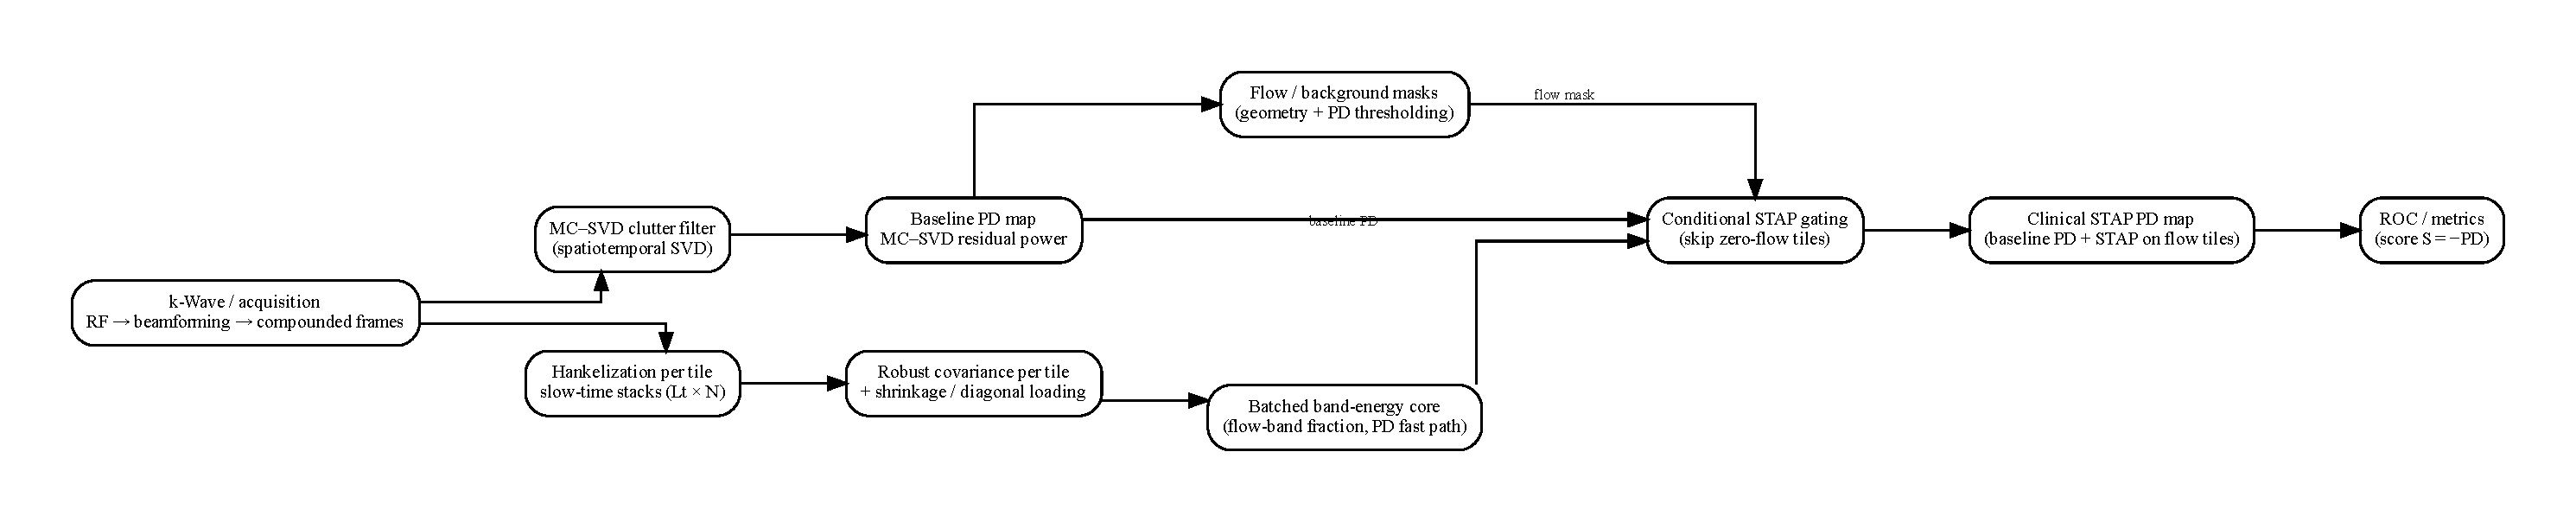
\includegraphics[width=\linewidth]{stap_pipeline.pdf}
  \caption{Block diagram of the clinical STAP PD pipeline. Starting from k-Wave simulations or acquired RF data, we form compounded frames and apply a motion-compensated SVD clutter filter to obtain a baseline PD map and flow/background masks. The temporal STAP core then operates on Hankelized slow-time tiles: robust per-tile covariances are estimated, conditioned, and used to whiten the slow-time snapshots; a batched band-energy kernel computes flow-band energy fractions. Conditional STAP gating applies this temporal STAP only on tiles that intersect the flow mask, while tiles with no flow support retain the baseline PD. The resulting STAP PD map is used as a detector with score $S=-\mathrm{PD}$ for ROC analysis.}
  \label{fig:stap_pipeline}
\end{figure}

\paragraph{Implementation summary.}
Algorithmically, the clinical STAP PD path used in all experiments can be summarized as follows:
\begin{itemize}[nosep]
  \item A motion-compensated SVD clutter filter is used as the baseline: for each volume we register frames to a reference, assemble a slow-time$\times$space Casorati matrix, and remove a low-rank tissue subspace chosen by an energy-fraction rule (``literature MC--SVD''), yielding a baseline PD map in $\approx 1$~s per 320-frame volume.
  \item The clinical STAP configuration fixes tile geometry (tiles of size $8\times 8$ with stride 3), a slow-time aperture $L_t=8$, conservative shrinkage and diagonal loading to keep temporal covariances well-conditioned, and a fixed Doppler band design (flow/alias bands and fd-grid) that is reused across regimes; a short slow-time window (roughly 200~ms) and a cap on Hankel snapshots per tile limit the effective training support.
  \item In the PD-focused fast path, the temporal STAP core builds Hankelized slow-time snapshots per tile, estimates a robust covariance for each tile, whitens the snapshots, and computes a flow-band energy fraction (matched-subspace statistic) in a fully batched way across tiles. These band fractions are then aggregated over slow time and combined with the baseline PD map to form the STAP PD map.
  \item Tiles are processed in GPU batches (typically on the order of a few hundred tiles per batch) to amortize Hankel construction, covariance estimation, and band-energy computation over many tiles while respecting memory limits.
  \item Conditional STAP gating uses the flow mask to decide where STAP is applied: tiles whose support contains no flow-mask pixels are not passed through STAP at all; instead they retain the baseline PD, while tiles with any flow-mask coverage receive the full STAP processing. This focuses STAP effort on the subset of tiles that can plausibly contain flow while leaving background tiles unchanged.
  \item The implementation records timing and coverage telemetry (number of tiles processed by STAP, number skipped, and per-phase runtimes for Hankel construction, covariance estimation, and band-energy computation) for every run; the latency and ROC summaries above are derived from this telemetry under the PD scoring mode with score $S=-\mathrm{PD}$.
\end{itemize}

\paragraph{Robustness sweeps (Phase 1.1).}
To quantify how stable the clinical STAP PD uplift is under realistic acquisition and tiling variations, we added a robustness-sweep driver (\texttt{scripts/run\_brain\_replay\_sweep.py}) and aggregator (\texttt{scripts/aggregate\_brain\_sweep.py}). The sweep spans Brain-OpenSkull and Brain-SkullOR pilots over PRF $\{1.2,1.5,2.0\}$~kHz, tile sizes $\{6\times 6,8\times 8,12\times 12\}$ with fixed strides $\{2,3,4\}$, slow-time apertures $L_t\in\{6,8,10\}$, and modest nuisance perturbations (clutter SNR offsets $\pm 3$~dB around the nominal brain SNR and alias amplitude scales $\{0.8,1.0,1.2\}$). For each configuration we reuse a k-Wave pilot per (regime, PRF), replay the clinical STAP PD profile on top of an MC--SVD baseline using \texttt{scripts/replay\_stap\_from\_run.py} (KA disabled), record per-volume latency and conditional-STAP coverage from \texttt{stap\_fallback\_telemetry}, and invoke \texttt{scripts/hab\_contract\_check.py} with \texttt{--score-mode pd} to extract TPR at FPR $\{10^{-4},3\times 10^{-4},10^{-3}\}$. The aggregator folds these runs into a matrix-style JSON/CSV table with $\Delta\mathrm{TPR}$ (STAP minus MC--SVD) and latency/coverage as functions of PRF, tile geometry, $L_t$, and nuisance scales.

Across all 243 sweep points per regime (OpenSkull and SkullOR) the MC--SVD PD baseline remains essentially flat in the extreme tail (TPR $\approx 0$ at FPR $10^{-4}$--$10^{-3}$), while the clinical STAP PD profile retains a nonzero shoulder with mean TPRs of roughly $0.19,0.24,0.38$ at FPR $10^{-4},3\times 10^{-4},10^{-3}$, respectively, and ranges $0.00$--$0.40$, $0.01$--$0.50$, and $0.03$--$0.71$ across the grid. This confirms that the PD uplift is not a single hyperparameter sweet spot but persists under moderate variation in PRF, tile geometry, $L_t$, clutter SNR, and alias amplitude.

The implementation follows this decomposition closely, with separate components for simulation, temporal STAP, and replay/analysis; the exact software layout is not essential to the methodology and is therefore omitted here. A schematic overview of this pipeline is shown in Figure~\ref{fig:stap_pipeline}.
For reproducible plots, we use an automated pipeline that regenerates the three canonical bundles (Brain-OpenSkull, Brain-AliasContract, Brain-SkullOR), recomputes PD-based contract checks, and produces latency bars and low-FPR ROC points corresponding to the summary in Table~\ref{tab:brain_latency}. The same pipeline also drives the full Brain-* suite end-to-end (pilot generation, baseline and STAP replays for MC--SVD/RPCA/HOSVD, ROC aggregation) so that the main simulated results and figures in this section can be regenerated in a single scripted run.

\section*{References}

\begin{thebibliography}{99}

\bibitem{Imbault2017}
Imbault, M., et al.
\newblock Intraoperative functional ultrasound imaging of human brain activity.
\newblock \emph{Scientific Reports} 7, 7304 (2017).

\bibitem{Mace2011}
Mac{\'e}, E., Montaldo, G., Pernot, M., Cohen, I., and Tanter, M.
\newblock Functional ultrasound imaging of the brain.
\newblock \emph{NeuroImage} 54(4), 2720--2731 (2011).

\bibitem{Urban2022}
Urban, A., et al.
\newblock In vivo whole brain microvascular imaging in mice using ultrafast ultrasound.
\newblock \emph{EBioMedicine} 76, 103861 (2022).

\bibitem{TCDVelocities}
Alexandrov, A. V., et al.
\newblock Velocity measurements in the middle cerebral arteries of healthy adults by transcranial Doppler.
\newblock \emph{Journal of Neuroimaging} 1, 166--172 (1991).

\bibitem{TCDOptimalFlow}
Alexandrov, A. V., et al.
\newblock Optimal values of flow velocity on transcranial Doppler in patients with intracranial arterial stenosis.
\newblock \emph{Stroke} 33, 1757--1761 (2002).

\bibitem{Mace2013}
Mac{\'e}, E., et al.
\newblock Functional ultrasound imaging of the brain: theory and basic principles.
\newblock \emph{IEEE Transactions on Ultrasonics, Ferroelectrics, and Frequency Control} 60(3), 492--506 (2013).

\bibitem{Rabut2020}
Rabut, C., et al.
\newblock Functional ultrasound imaging of human brain activity through the skull.
\newblock \emph{Science Translational Medicine} 12(572), eaav4392 (2020).

\bibitem{Rabut2024}
Rabut, C., Norman, S. L., Griggs, W. S., Russin, J. J., Jann, K., et al.
\newblock Functional ultrasound imaging of human brain activity through an acoustically transparent cranial window.
\newblock \emph{Science Translational Medicine} 16(572), eadj3143 (2024).

\bibitem{Deffieux2021}
Deffieux, T., Demen{\'e}, C., and Tanter, M.
\newblock Functional ultrasound imaging: A new imaging modality for neuroscience.
\newblock \emph{Neuroscience} 474, 110--121 (2021).

\bibitem{Demeulenaere2022}
Demeulenaere, O., Bertolo, A., Pezet, S., Osmanski, B.-F., Tanter, M., and Deffieux, T.
\newblock In vivo whole brain microvascular imaging in mice using transcranial 3D ultrasound localization microscopy.
\newblock \emph{EBioMedicine} 79, 103995 (2022).

\bibitem{ICDFUS2021}
Demene, C., et al.
\newblock Improved color Doppler for cerebral blood flow axial velocity estimation (iCD-fUS).
\newblock \emph{IEEE Transactions on Medical Imaging} 40(5), 1498--1510 (2021).

\bibitem{Tang2021}
Tang, J., Kilic, K., Szabo, T. L., and Boas, D. A.
\newblock Improved color Doppler for cerebral blood flow axial velocity imaging.
\newblock \emph{IEEE Transactions on Medical Imaging} 40(2), 758--764 (2021).

\bibitem{MobileFUS2024}
Urban, A., et al.
\newblock Mobile human brain imaging using functional ultrasound.
\newblock \emph{Nature Biomedical Engineering} 8, 534--546 (2024).

\bibitem{Aaslid1982}
Aaslid, R., Markwalder, T.-M., and Nornes, H.
\newblock Noninvasive transcranial Doppler ultrasound recording of flow velocity in basal cerebral arteries.
\newblock \emph{Journal of Neurosurgery} 57(6), 769--774 (1982).

\bibitem{Gao2002}
Gao, S., Lam, W. W.-K., Chan, Y.-H., Liu, J., Wong, K.-P., Leung, T. W.-S., et al.
\newblock Optimal values of flow velocity on transcranial Doppler in grading middle cerebral artery stenosis in comparison with magnetic resonance angiography.
\newblock \emph{Journal of Neuroimaging} 12(3), 213--218 (2002).

\bibitem{Estrada2018}
Estrada, H., Gottschalk, S., Reiss, M., Neuschmelting, V., Razansky, D., et al.
\newblock Observation of guided acoustic waves in a human skull.
\newblock \emph{Ultrasound in Medicine \& Biology} 44(7), 1438--1447 (2018).

\bibitem{CandesRPCA}
Cand{\`e}s, E. J., Li, X., Ma, Y., and Wright, J.
\newblock Robust principal component analysis?
\newblock \emph{Journal of the ACM} 58(3), 11 (2011).

\bibitem{LinALM}
Lin, Z., Chen, M., and Ma, Y.
\newblock The augmented Lagrange multiplier method for exact recovery of corrupted low-rank matrices.
\newblock \emph{arXiv preprint} arXiv:1009.5055 (2010).

\bibitem{HalkoRandomizedSVD}
Halko, N., Martinsson, P. G., and Tropp, J. A.
\newblock Finding structure with randomness: Probabilistic algorithms for constructing approximate matrix decompositions.
\newblock \emph{SIAM Review} 53(2), 217--288 (2011).

\bibitem{LampeFUSBrain}
\newblock Functional ultrasound imaging of the brain.
\newblock UNC/NCSU Joint Department of Biomedical Engineering teaching material, online resource, accessed 2024.
\newblock Available at \url{https://bme.unc.edu/wp-content/uploads/sites/917/2021/08/functional_ultrasound.pdf}.

\bibitem{MCAFlowsCombinedTCD}
\newblock Middle cerebral artery blood flows by combining TCD with complementary measurements.
\newblock Online resource, accessed 2024.
\newblock Available at \url{https://pmc.ncbi.nlm.nih.gov/articles/PMC4609642/}.

\bibitem{RealTimeRandomizedSVD}
\newblock Real-time SVD-based clutter filtering using randomized singular value decomposition.
\newblock Online resource, accessed 2024.
\newblock Available at \url{https://pmc.ncbi.nlm.nih.gov/articles/PMC7293562/}.

\bibitem{Soloukey2020FUSAwake}
Soloukey, S., Vincent, A. J. P. E., Smits, M., Slump, C. H., Dirven, C. M. F., et al.
\newblock Functional ultrasound (fUS) during awake brain surgery: the clinical potential for intra-operative functional and vascular brain mapping.
\newblock \emph{Frontiers in Neuroscience} 13, 1384 (2019).
\newblock Available at \url{https://www.frontiersin.org/articles/10.3389/fnins.2019.01384}.

\bibitem{FUSLocMicro}
\newblock Functional ultrasound localization microscopy reveals brain vessel activity at micron-scale resolution.
\newblock Online resource, accessed 2024.
\newblock Available at \url{https://pmc.ncbi.nlm.nih.gov/articles/PMC9352591/}.

\bibitem{HamdanHumanFUS}
\newblock Functional ultrasound imaging of human brain activity through skull.
\newblock Online resource, accessed 2024.
\newblock Available at \url{https://www.vis.caltech.edu/documents/28341/scitranslmed.adj3143.pdf}.

\bibitem{PhaseAberrationCorrection}
\newblock Rapid full-wave phase aberration correction method for transcranial ultrasound.
\newblock Online resource, accessed 2024.
\newblock Available at \url{https://jtultrasound.biomedcentral.com/articles/10.1186/s40349-016-0074-7}.

\bibitem{UltrafastUltrasoundBook}
\newblock Ultrafast Ultrasound Imaging.
\newblock Online resource, accessed 2024.
\newblock Available at \url{https://mdpi-res.com/bookfiles/book/756/Ultrafast_Ultrasound_Imaging.pdf}.

\bibitem{StaggeredPRFColorDoppler}
\newblock Staggered multiple-PRF ultrafast color Doppler.
\newblock Online resource, accessed 2024.
\newblock Available at \url{https://www.biomecardio.com/publis/ieeetmi16.pdf}.

\bibitem{FunctionalFUSBrain}
\newblock Functional ultrasound imaging: a useful tool for neuroscience.
\newblock Online resource, accessed 2024.
\newblock Available at \url{https://www.sciencedirect.com/science/article/pii/S1053811921009940}.

\bibitem{MaceWholeBrainZenodo}
Mac{\'e}, E., Urban, A., and Tanter, M.
\newblock Whole-brain visually evoked activity maps in head-fixed awake mice.
\newblock Zenodo dataset, DOI 10.5281/zenodo.4905862 (2021).

\bibitem{FUSBMIData}
Griggs, W. S., et al.
\newblock Dataset for: Decoding motor plans using a closed-loop ultrasonic brain–machine interface.
\newblock CaltechDATA record, DOI 10.22002/pa710-cdn95 (2024).

\bibitem{WindowCaltechData}
Rabut, C., et al.
\newblock Dataset for: A window to the brain: ultrasound imaging of human neural activity through an acoustically transparent cranial prosthetic.
\newblock CaltechDATA record, DOI 10.22002/f3y3k-em558 (2023).

\bibitem{WangULMZenodo}
Wang, Y., et al.
\newblock Longitudinal awake imaging of mouse deep brain microvasculature with super-resolution ultrasound localization microscopy.
\newblock Zenodo dataset, DOI 10.5281/zenodo.17393921 (2024).

\bibitem{WangULMELife}
Wang, Y., et al.
\newblock Longitudinal awake imaging of mouse deep brain microvasculature with super-resolution ultrasound localization microscopy.
\newblock \emph{eLife} 14, e95168 (2025).

\bibitem{AcceleratedSVDUltrasound}
\newblock Accelerated singular value-based ultrasound blood flow clutter filtering.
\newblock Online resource, accessed 2024.
\newblock Available at \url{https://scispace.com/papers/accelerated-singular-value-based-ultrasound-blood-flow-qofwd4rmcy}.

\bibitem{SVDClutterFilterReview}
\newblock On the use of singular value decomposition as a clutter filter for ultrasound flow imaging.
\newblock Online resource, accessed 2024.
\newblock Available at \url{https://www.researchgate.net/publication/370263218_On_the_Use_of_Singular_Value_Decomposition_as_a_Clutter_Filter_for_Ultrasound_Flow_Imaging}.

\bibitem{UltrafastRPCAClutter}
\newblock Ultrafast online clutter filtering for ultrasound blood flow imaging using robust principal component analysis.
\newblock Online resource, accessed 2024.
\newblock Available at \url{https://pubmed.ncbi.nlm.nih.gov/40031320/}.

\bibitem{AdaptiveHOSVDClutter}
\newblock Adaptive higher-order singular value decomposition clutter filtering for ultrasound flow imaging.
\newblock Online resource, accessed 2024.
\newblock Available at \url{https://pure.tue.nl/ws/portalfiles/portal/337451900/1-s2.0-S0041624X24000696-main.pdf}.

\end{thebibliography}

\subsection{Practical Band Design for Brain fUS (PRF $\approx$ 1.5--5 kHz, $T\approx 8$--16)}

Finally, we keep the practical band guidelines, adding explicit physical anchors.

For brain fUS at center frequencies $f_0 \approx 6$--$15$ MHz and PRF $\approx 1.5$--$5$ kHz \cite{Mace2013,Rabut2020,Imbault2017,Urban2022,LampeFUSBrain}:

\begin{itemize}[nosep]
  \item Microvascular brain flows (arterioles/venules) in humans and rodents are typically in the range $v \approx 3$--$20$ mm/s for the vessels that dominate functional responses \cite{Imbault2017,Urban2022}. At $f_0=7.5$ MHz and $c\approx 1540$ m/s, this corresponds to Doppler shifts $f_D\approx 30$--$200$ Hz.
  \item Low--frequency tissue motion (respiration, cardiac pulsation) produces strong spectral content below $\approx 20$ Hz; this should be contained in Po and largely removed by high--pass filtering and/or SVD.
  \item Large--vessel flows (e.g.\ MCA--like arteries) reach $v\approx 0.3$--$0.8$ m/s, corresponding to $f_D$ in the kHz range \cite{TCDVelocities,TCDOptimalFlow,MCAFlowsCombinedTCD}. Depending on PRF and angle, a portion of this energy appears in high Doppler bands and can alias into the $>$400 Hz region corresponding to Pa \cite{ICDFUS2021,MobileFUS2024}.
\end{itemize}

Thus a reasonable fixed band design for brain fUS with $T\approx 8$--$16$ and PRF $\approx 1.5$--$3$ kHz is:

\begin{itemize}[nosep]
  \item Flow band $\Cf$: $[30,250]$ Hz --- microvascular flows $\approx 3$--$20$ mm/s.
  \item Guard band $\Cg$: $[250,400]$ Hz --- protects against band--edge leakage.
  \item Alias band $\Ca$: $[400, \text{Nyquist}]$ Hz --- high Doppler where large--vessel/aliased flows and certain motion artifacts live.
\end{itemize}

In discrete terms, for $T=8$ at PRF=1.5 kHz (bin spacing $187.5$ Hz), this maps to:
\begin{itemize}[nosep]
  \item $\Pf$ on first off--DC bin (with DPSS leakage covering $\approx 30$--$250$ Hz),
  \item guard around the second bin,
  \item $\Pa$ on higher bins with bin--level guard as per BG--1/BG--2.
\end{itemize}

\section{Additional real-data stress tests}\label{app:negative-real}
\paragraph{Wang ULM IQ (awake mouse).} We load the authors' IQData files exactly as in \texttt{LoadIQ.m} (column-major reshape) and build a coarse vessel/background prior on the native $320\times 161$ grid via a simple temporal high-pass (second difference or removal of a few leading temporal singular modes), high-quantile thresholding, and accumulation; when no prior is provided we fall back to PD-mean quantiles. We then apply the frozen clinical STAP PD core (tiles $8\times 8$, stride~3, $L_t=8$--$16$, Pf/Pa/guard bands scaled to kHz PRF) on 256-frame windows across all IQ files and record Pf/Pa peak fractions, alias ratios, and PD-z ROC at low FPR. On all files and windows Pf never dominates (Pf peak fraction $\approx 0$), Pa/Po absorb most energy, and PD-z ROC remains weak; widening bands or adjusting $dt$ (0.001--0.002~s) does not change this. We interpret Wang as already heavily compounded/filtered (PD-like), with the Doppler precondition R--1 failing; it serves only as a conservative contract sanity check.

\paragraph{PICMUS carotid RF (in vivo plane-wave).} Using the publicly hosted UFF carotid cross-section data, we implement a delay-and-sum beamformer to produce an IQ/PD cube and apply the same Doppler STAP configuration scaled to its $\approx 100$ Hz PRF. Slow-time energy lies near DC, Pf/Pa never dominate, alias metrics show no class separation, and PD-z/BR/GLRT ROCs are flat. We therefore classify PICMUS as out of regime for the fixed clinical Doppler profile and use it only as a stress test demonstrating that the contract telemetry correctly withholds KA/STAP claims when Pf/Pa structure is absent.

\section{Algorithmic details (supplementary)}
\label{app:alg-details}

\section{Simulation details (supplementary)}
\label{app:sim-details}

Full depth-zone definitions, amplitude/coverage tuning, alias/vibration components, motion/aberration models, and replay settings for all Brain-* profiles (OpenSkull, Pial128, AliasContract, SkullOR) are provided here for completeness; the main text retains only the regime summary table and short role descriptions.

\section{Implementation details (supplementary)}
\label{app:impl-details}

\subsection{RPCA baseline (full)}
All steps for the RPCA/PCP baseline, including spatial downsampling, temporal windowing, matrix formation, IALM updates, stopping criteria, and PD reconstruction, are documented here.

\subsection{HOSVD baseline (full)}
Mode-unfolding, truncated SVDs, energy-based rank caps, low-rank projection, and PD reconstruction details for the HOSVD/Tucker baseline appear here.

\subsection{STAP temporal core (full)}
Hankel construction shapes, batching strategy, robust covariance estimators, whitening, band-energy computation, and the PD-only fast path and conditional STAP logic are detailed here.

\subsection{Covariance blending constraints and KA modes}

We permit anisotropic shrinkage, but only \emph{within} bands. In practice we consider two KA paths:
\begin{itemize}[nosep]
  \item \textbf{Updated (commuting band--scalar).} $Q^\top Q$ is forced to be bandwise scalar with target gains $(s_f,s_a,s_o)$ (in code: $s_f=s_o\approx 1$, $s_a\approx 1.5$), small mixing, and no off--block priors; the content of $R_0$ beyond $(\Pf,\Pa)$ is ignored.
  \item \textbf{Blend.} A trace--normalized blend $R_\beta = (1-\beta) R_t^{(n)} + \beta R_0^{(n)}$ with a small diagonal lift. In practice $R_0$ is overridden to a band--scalar form (Pf weight 1, Pa weight $\gamma_a>1$, Po weight 1) so the geometry is explicit; $\beta$ is treated as a fixed hyperparameter per regime.
\end{itemize}
Both modes enforce bandwise structure; there are no off--block priors.

\subsection{CB--1: Band--Block Blending}

We construct
\[
R_\beta := (1-\beta)\,\wh R + \beta \bigl(R_{0,f}\oplus R_{0,a}\oplus R_{0,o}\bigr) + \delta I,
\]
where $R_{0,f} = \Pf R_0 \Pf$, etc., for some prior $R_0$. There are no off--block priors; $\beta\in[0,1)$ and $\delta\ge 0$.

Interpretation: this structure makes $Q$ nearly block--diagonal in $(\Pf,\Pa,\Po)$ while still allowing bandwise control to realize OC--2.

\subsection{CB--2: Bandwise Spectral Targets}

We choose $(\beta,\delta)$ to enforce OC--2 explicitly:
\[
\lambda_{\min}(Q^\top Q|_{\Pf}) \in [s_f^2(1-\delta_f), s_f^2(1+\delta_f)],\quad\text{etc.}
\]
with design tolerances $\delta_\bullet\le 0.1$ and separation $\Lambda = s_a/s_f \ge 1.25$.

\subsection{CB--3: Bandwise Condition Number Safeguard}

We constrain bandwise conditioning:
\[
\kappa(R_\beta|_{\Pf}) \le \kappa_f^{\max},\qquad
\kappa(R_\beta|_{\Pa}) \le \kappa_a^{\max},
\]
avoid an incompatibility between conditioning and preserving flow Rayleigh quotients.

\subsection{Gating (localizing KA in score space)}
\label{app:gating}

A global band--constant transform with $Q$ cannot improve ROC if applied everywhere (it is close to a scalar reweighting of BR/GLRT). To create re--ranking, KA must be \emph{localized} to tiles where:
\begin{itemize}[nosep]
  \item scores are dominated by alias/undesired components,
  \item positives are unlikely to lie.
\end{itemize}

We define gating based on a combination of alias metrics, flow coverage, depth, PD, and registration. This supplements G--1/G--2 with a generalized alias score $m_{\text{alias}}$ from Section~\ref{sec:regime}.

\subsection{G--1: Alias--dominant tile selection}

Given a baseline tile $z$, compute per--band energies $(E_f,E_a,E_g,E_{\text{dc}})$ and a generalized alias score $m_{\text{alias}}(z)$ satisfying R--2.

\paragraph{Data--adaptive threshold.}
For BG tiles (or their proxy), collect $m_{\text{alias}}(z)$ and define
\[
\tau_{\text{alias}} := Q_{q_{\text{alias}}}\bigl(m_{\text{alias}} \mid H_0\bigr),
\]
where $Q_q$ is the $q$--quantile and $q_{\text{alias}}\in[0.7,0.9]$ is a design choice (typical: $0.8$ or $0.9$).

Define an alias gate
\[
g_{\text{alias}}(z) = \mathbf{1}\left\{ m_{\text{alias}}(z) \ge \tau_{\text{alias}} \right\}.
\]

\paragraph{Band--edge purity.}
Additionally require that guard energy is small relative to Pf+Pa:
\[
\frac{E_g}{E_f + E_a + E_g + E_{\text{dc}}} \le \eta_{\text{edge}},\quad
\eta_{\text{edge}}\le 0.1.
\]

Interpretation: this gate selects the top tail of alias--heavy tiles among negatives, while protecting against band--edge contamination. The distribution of $m_{\text{alias}}$ across classes is governed by R--2; empirical validation (Section~\ref{sec:regime}) must show a nontrivial difference between $H_0$ and $H_1$.

\subsection{G--2: Flow coherence veto}

We can optionally compute a flow coherence metric $\mathrm{FPC}$ (first principal component fraction) within the flow band:
\[
\mathrm{FPC} := \frac{\lambda_1(\wh S_f)}{\tr(\wh S_f)},\qquad
\wh S_f := \frac{1}{K}\sum_{k=1}^K u_k u_k^\top,\quad
u_k := \Pf z^{(k)},
\]
where $z^{(k)}$ are projected slow--time vectors across DPSS tapers or within a local ensemble.

Gate \emph{may} require
\[
\mathrm{FPC}\le c_{\text{pc}},\qquad c_{\text{pc}}\in[0.4,0.6].
\]

Interpretation: flow tiles tend to exhibit higher coherence in Pf; when enabled, we veto gating when $\mathrm{FPC}$ is large, thereby reducing positive gating probability $p_+$. Alias/motion tiles have lower flow coherence and pass this condition. In the current acceptance runs this check is typically left off; coverage and depth gating carry most of the class separation.

\subsection{G--2': Flow coverage veto}

Let $c_f$ be the tile--wise flow coverage fraction:
\[
c_f := \frac{\#\{\text{pixels labeled as flow}\}}{\#\{\text{pixels in tile}\}},
\]
using a label--free proxy such as a PD--derived flow mask.

We require
\[
c_f \le c_{f,\max},\qquad c_{f,\max}\in[0.1,0.2],
\]
and optionally $c_f \ge c_{f,\min}$ to avoid pure background noise tiles (typical $c_{f,\min}\approx 0$).

Interpretation: we prefer gating on tiles with \emph{low to moderate} flow coverage. This is the regime where alias/motion dominates and where down--scaling scores is most beneficial. Dense flow tiles are either left to STAP alone or are guarded via the flow coherence veto. (In the current implementation, coverage is treated as an \emph{upper} bound; missing coverage defaults to ``pass'' in this test.)

\subsection{G--3: Baseline score quantile window}

Let $S_{\text{base}}(z)$ be the baseline BR/GLRT score. Within a given depth stratum, compute score quantiles $q_{0.3},q_{0.95}$ over BG tiles. Gate requires
\[
S_{\text{base}}(z)\in [q_{0.3},q_{0.95}].
\]

Interpretation: avoid gating on the noise floor (very low scores) and on already high--confidence positives (very high scores). This focuses KA on the part of the negative tail that matters near the target FPR.

\subsection{G--4: Registration quality (optional)}

If motion compensation / registration is used, include a registration quality metric (e.g.\ PSR) and require
\[
\mathrm{PSR}_{\text{reg}}\le \text{PSR}_{\max},
\]
or any similar condition ensuring that tiles with gross registration failure are handled separately.

\subsection{Offline validation of gating}

On a held--out labeled configuration, define
\[
p_+ := \mathbb{P}\{g=1\mid H_1\},\qquad
p_- := \mathbb{P}\{g=1\mid H_0\},
\]
for the combined gate $g$ that incorporates G--1, G--2, G--2', G--3, G--4. Require:
\[
p_-\ge 0.2,\quad p_- \le 0.5,\quad p_+ \le 0.1 p_-.
\]

Interpretation: a nontrivial fraction of negatives are gated (but not too many), while positives are rarely gated. This condition is central to the SL--2 quantile shift argument.

\subsection{Summary: Compact Feasibility Checklist (Updated)}

KA--STAP can be expected to outperform MC--SVD (or STAP--only) at low FPR if and only if:

\begin{enumerate}[label=\arabic*.,nosep]
  \item \textbf{Regime preconditions.} Band occupancy R--1, alias separation R--2, and baseline headroom R--3 are satisfied on a held--out validation set.
  \item \textbf{Band design.} BG--1/BG--2/BG--3 hold for the chosen PRF/$T$/DPSS; Pf/Pa are physically meaningful (e.g.\ Pf $\approx$ 30--250 Hz, Pa $\gtrsim$ 400 Hz in brain fUS).
  \item \textbf{Operator geometry.} OC--1 with $\varepsilon_{\text{mix}}\le 0.05$ and OC--2 with $\Lambda = s_a/s_f \ge 1.25$ and $\delta_\bullet\le 0.1$.
  \item \textbf{Blending realizable.} CB--1/CB--2/CB--3 satisfied with chosen $(\beta,\delta)$.
  \item \textbf{Gating conservative and class--differential.} G--1/G--2/G--2'/G--3/G--4 implemented; offline, $p_-\in[0.2,0.5]$ and $p_+\le 0.1p_-$.
  \item \textbf{Regime sentinel.} RS--1 does not trigger (KA not out of regime).
  \item \textbf{Invariance sentinel.} $\wh s_a/\wh s_f \notin[1-\epsilon,1+\epsilon]$ with $\epsilon\le 0.02$; otherwise KA is effectively scalar and can be skipped.
  \item \textbf{Safety guard.} Safety--1 (monotonicity on gated flow tiles) passes.
  \item \textbf{Evaluation discipline.} GLRT controls and tail CI practices (Section~\ref{sec:eval}) in place for fair low--FPR comparison.
\end{enumerate}

When all of the above hold, KA applies a non--mixing, alias--inflating band transform chiefly to alias--dominant tiles, pushing negative scores down while largely leaving positives unchanged. This lowers the negative $\alpha$--quantile and increases TPR at fixed small FPR in a manner consistent with the SL--2 quantile shift analysis.

\begin{thebibliography}{9}
\bibitem{Capon1969Beamformer}
J. Capon, ``High-resolution frequency-wavenumber spectrum analysis,'' \emph{Proc. IEEE}, vol. 57, no. 8, pp. 1408--1418, 1969.

\bibitem{FrostBeamformer}
O. L. Frost, ``An algorithm for linearly constrained adaptive array processing,'' \emph{Proc. IEEE}, vol. 60, no. 8, pp. 926--935, 1972.

\bibitem{WardSTAPTutorial}
J. Ward, ``Space-time adaptive processing for airborne radar,'' MIT Lincoln Lab, Tech. Rep. 1015, Dec. 1994.
\end{thebibliography}

\end{document}
